% Options for packages loaded elsewhere
\PassOptionsToPackage{unicode}{hyperref}
\PassOptionsToPackage{hyphens}{url}
%
\documentclass[
  12pt,
]{article}
\usepackage{amsmath,amssymb}
\usepackage{iftex}
\ifPDFTeX
  \usepackage[T1]{fontenc}
  \usepackage[utf8]{inputenc}
  \usepackage{textcomp} % provide euro and other symbols
\else % if luatex or xetex
  \usepackage{unicode-math} % this also loads fontspec
  \defaultfontfeatures{Scale=MatchLowercase}
  \defaultfontfeatures[\rmfamily]{Ligatures=TeX,Scale=1}
\fi
\usepackage{lmodern}
\ifPDFTeX\else
  % xetex/luatex font selection
\fi
% Use upquote if available, for straight quotes in verbatim environments
\IfFileExists{upquote.sty}{\usepackage{upquote}}{}
\IfFileExists{microtype.sty}{% use microtype if available
  \usepackage[]{microtype}
  \UseMicrotypeSet[protrusion]{basicmath} % disable protrusion for tt fonts
}{}
\makeatletter
\@ifundefined{KOMAClassName}{% if non-KOMA class
  \IfFileExists{parskip.sty}{%
    \usepackage{parskip}
  }{% else
    \setlength{\parindent}{0pt}
    \setlength{\parskip}{6pt plus 2pt minus 1pt}}
}{% if KOMA class
  \KOMAoptions{parskip=half}}
\makeatother
\usepackage{xcolor}
\usepackage[margin=1in]{geometry}
\usepackage{graphicx}
\makeatletter
\def\maxwidth{\ifdim\Gin@nat@width>\linewidth\linewidth\else\Gin@nat@width\fi}
\def\maxheight{\ifdim\Gin@nat@height>\textheight\textheight\else\Gin@nat@height\fi}
\makeatother
% Scale images if necessary, so that they will not overflow the page
% margins by default, and it is still possible to overwrite the defaults
% using explicit options in \includegraphics[width, height, ...]{}
\setkeys{Gin}{width=\maxwidth,height=\maxheight,keepaspectratio}
% Set default figure placement to htbp
\makeatletter
\def\fps@figure{htbp}
\makeatother
\setlength{\emergencystretch}{3em} % prevent overfull lines
\providecommand{\tightlist}{%
  \setlength{\itemsep}{0pt}\setlength{\parskip}{0pt}}
\setcounter{secnumdepth}{5}
\usepackage{float}
\usepackage{sectsty}
\usepackage{paralist}
\usepackage{setspace}
\usepackage{fancyhdr}
\usepackage{lastpage}
\usepackage{dcolumn}
\usepackage{chemformula}
\usepackage{chemmacros}
\usepackage{natbib}\bibliographystyle{agsm}
\usepackage[nottoc, numbib]{tocbibind}
\usepackage{booktabs}
\ifLuaTeX
  \usepackage{selnolig}  % disable illegal ligatures
\fi
\IfFileExists{bookmark.sty}{\usepackage{bookmark}}{\usepackage{hyperref}}
\IfFileExists{xurl.sty}{\usepackage{xurl}}{} % add URL line breaks if available
\urlstyle{same}
\hypersetup{
  pdftitle={Masters Thesis: Coded in R},
  pdfauthor={Robert J. Dellinger},
  hidelinks,
  pdfcreator={LaTeX via pandoc}}

\title{Masters Thesis: Coded in R}
\author{\href{https://robdellinger.com}{Robert J. Dellinger}}
\date{2024}

\begin{document}
\maketitle

\newpage
\pagestyle{empty}

\allsectionsfont{\centering}
\subsectionfont{\raggedright}
\subsubsectionfont{\raggedright}

\begin{centering}

\vspace{1 in}
{\bf CALIFORNIA STATE UNIVERSITY, NORTHRIDGE}

\vspace{0.1 in}
{Department of Biology}
\vspace{0.2 in}




\includegraphics[width=0.3\linewidth]{Images/university_logo} 


\vspace{0.1 in}

\doublespacing
{\bf Facing Physiological Constraints: Investigating the Interactive Effects of Ocean Acidification and Warming on the Metabolic Demand of an Intertidal Gastropod \emph{Tegula funebralis} Amidst a Fluctuating Tidal Environment \\}

\vspace{0.3 in}

Thesis submitted in partial fulfillment of the requirements\\
For the degree of Master of Science in Biology \\

\vspace{0.4 in}
\singlespacing
By

\vspace{0.1 in}
{Robert J. Dellinger}

\vspace{2 in}
May 2024

\end{centering}
\doublespacing

\newpage
\pagestyle{plain}
\pagenumbering{roman}

\section*{}

\vfill

\begin{center}
Copyright by Robert J. Dellinger
\end{center}

\newpage

The thesis of Robert J. Dellinger is approved:

\vspace{1.5in}

\underline{\hspace{2.5in}}\hspace{0.5in} \underline{\hspace{2in}}

Dr.~Peter J. Edmunds \hspace{1.65in} Date:

\vspace{0.5in}

\underline{\hspace{2.5in}}\hspace{0.5in} \underline{\hspace{2in}}

Dr.~Kerry J. Nickols \hspace{1.75in} Date:

\vspace{0.5in}

\underline{\hspace{2.5in}}\hspace{0.5in} \underline{\hspace{2in}}

Dr.~Nyssa J. Silbiger, Chair \hspace{1.3in} Date:

\vfill

\begin{center}
California State University, Northridge
\end{center}

\newpage

\vspace*{\fill}

\begin{center}

\begin{minipage}{0.8\textwidth}
\begin{quote}

``Against this cosmic background the lifetime of a particular \\
  plant or animal appears, not as a drama complete in itself, \\
  but only as a brief interlude in a panorama of endless change.'' \\

— Rachel Carson, \textit{Undersea} (1937)
\end{quote}
\end{minipage}

\vspace*{\fill}

\begin{minipage}{0.8\textwidth}
\begin{quote}
``For nothing is fixed, forever, forever, forever, \\
  it is not fixed; \\
  the earth is always shifting, \\
  the light is always changing, \\
  the sea does not cease to grind down rock.\\
  Generations do not cease to be born,\\ 
  and we are responsible to them \\
  because we are the only witnesses they have. \\
 
  The sea rises, the light fails, \\
  lovers cling to each other, \\
  and children cling to us. \\
  The moment we cease to hold each other, \\
  the moment we break faith with one another, \\
  the sea engulfs us and the light goes out.'' \\


— James Baldwin, \textit{Nothing Personal} (1964)
\end{quote}
\end{minipage}

\vspace*{\fill}

\end{center}

\newpage

\section*{Acknowledgements}

~~~~~ First and foremost, I would like to express my gratitude to our
ocean for the generosity it bestows upon us daily and for the awe it
instilled in me as a young child---a wonder that has grown into a
lifelong dream and pursuit. I am deeply grateful to Dr.~Nyssa J.
Silbiger, my advisor, for her unwavering support, encouragement,
inspirational attitude, and collaboration on this project. Thank you for
believing in me, urging me to become the person I need to be, equipping
me with the knowledge, tools, and skills needed to achieve this, and for
ignoring the lies we often tell ourselves about ourselves. To my thesis
committee, Dr.~Peter J. Edmunds and Dr.~Kerry J. Nickols, thank you for
your invaluable guidance and advice throughout this process. Thank you
to my mentors, Dr.~Aradhna Tripati, Dr.~Rachel Bay, Dr.~Tessa Hill, and
Dr.~Melanie Okoro, who have acted as academic mothers, paving the way
and uplifting me throughout my academic trajectory. I would also like to
extend my gratitude to the Silbiger and Nichols Lab team, including D.M.
Barnas, J.R. Kerlin, C. Fajardo, and H. Merges. In particular, I want to
give a special thank you to J.B. Fields and T. Smith for their
monumental support and dedication in ensuring that everything ran
smoothly inside and outside of the lab; they were always there as
friends to call on and played pivotal roles in ensuring the success of
my degree. Without all of you, none of this would have been possible.
Throughout endless sleepless nights and days of struggle, thank you for
lifting as you climbed. A special thank you to Ana and the rest of the
custodial staff, whose skills are the cornerstone of the entire
institution, and whose presence makes the halls of academia feel more
like home as they sweep through the halls, serenaded by the rhythm of
bachata. This research couldn't have been possible without the financial
support from the National Science Foundation Graduate Research
Fellowship Program, UCLA Center for Diverse Leadership in Science Early
Career Fellowship, UC Davis Sustainable Oceans Scholars Program, and the
National Science Foundation CAREER grant OCE-2044837 awarded to
Dr.~Nyssa Silbiger, the material in this study based upon work supported
by the U.S. National Science Foundation, the CSUN Department of Biology,
and research activities that were conducted under scientific collecting
permits issued by the California Department of Fish and Wildlife (ID:
S-220520002-22054-001).

~~~~~ I extend my heartfelt gratitude to my family, Robert K. Dellinger
and Ana. C. Dellinger, for instilling in me the belief that education is
the most powerful tool. They have made me feel capable of achieving
anything I set my mind to and have unwaveringly supported my dreams,
regardless of their nature. To my father, thank you for raising me with
the understanding that everything we create must be done with love; love
is the secret ingredient. To my mother, I am forever thank you for
sacrificing your own dreams and for persevering through the challenges
of the ingratitude of the nation in which you settled, all to ensure
that I could pursue my own dreams and aspirations.Thank you to all of
those who have parented me and the push of the universe for laughing at
me. Thank you to my chosen family, including my partner and friends, who
immersed me in a queerness that dominant systems cannot understand, who
illuminated alternative paths from the outdated paradigms we are
entangled in, and who remember to swim despite everything. Their love
and resilience have nurtured me and imbued me with the buoyancy and
fortitude to demand better from the world around me. Thank you for your
willingness to churn the waters up, for being holders of wisdom and
knowledge, and for showing me that the facts of nature often falsify the
prevailing theories. I would not be here today without their love and
support.

~~~~~ Being a part of the CSUN and the Los Angeles community the past
three years has been some of the most formative and fulfilling
experiences of my life and for my career moving forward. Studying
climate change in an era marked by rapid ecological change and numerous
interconnected crises, encompassing racial capitalism and the climate
emergency, particularly during a time in which society stands at a
pivotal crossroads for humanity's future can feel rather dismal. Yet the
support and knowledge I've received from my community and mentors as
well as the collective imagination of the communities I am a part of has
instilled within me an unbridled sense of optimism. That amid these
challenges, we possess all of the solutions to the crises we face, and
that within our collectivities, there are reservoirs of hope for the
future - a future where our individual lives matter not less, but more,
as they form the pixels shaping a panorama of endless change.

\centering
\raggedright
\newpage
\tableofcontents

\newpage
\listoftables

\newpage
\listoffigures
\newpage

\pagenumbering{arabic}

\section*{Abstract}

Ocean acidification (OA) is occurring across a backdrop of concurrent
environmental changes that will reverberate to affect energy flow
throughout ecological communities. Ocean acidification and warming will
profoundly affect marine organisms, the ecosystems that organisms are
embedded within, and the services and functions ecosystems provide to
humanity. However, a mechanistic understanding of the interactive
effects of ocean acidification and warming on organismal physiology
remains a critical gap of uncertainty in a field that has prioritized a
reductionist approach to studying future oceanic scenarios as isolated
phenomena. The highly variable coastal environment of the rocky
intertidal, and the organisms within the ecosystem, provide a model
system to understand the physiological mechanisms for how organisms
respond to environmental change. To address these limitations, we used
thermal performance curves to empirically characterize the relationship
between biological rates of respiration and grazing of
\textit{Tegula funebralis}, an intertidal herbivore ubiquitous to the
highly variable rocky intertidal ecosystems of California. This study
measured thermal performance across a range of eight temperatures
crossed with a blocked exposure to either current average
(\(7.9 \pm 0.1\)) or future (\(7.7 \pm 0.8\)) average oceanic pH
predictions. Measurements for respiration rates were taken after a
10-day exposure thereby enabling us to quantify energetic expenditure.
Our results show no statistical difference between thermal performance
metrics (\(T_{\text{opt}}\), \(R_{\text{max}}\), \(CT_{\text{min}}\),
\(CT_{\text{max}}\)), yet there were differences in energy expenditure
between the high and low pH treatments as temperature increased. Our
results empirically characterize how measurements of performance will
respond to ocean warming and acidification and exemplify how
organismal-level interactions may scale up to affect different ecosystem
functions.

\newpage

\hypertarget{organism-physiology-in-response-to-multiple-drivers-of-environmental-change}{%
\section{Organism Physiology in Response to Multiple Drivers of
Environmental
Change}\label{organism-physiology-in-response-to-multiple-drivers-of-environmental-change}}

~~~~~ Organisms and environments are entwined, as the relationship
between organisms and the environments they are embedded within, is in
constant flux through inextricable links and flows of energy. The
relationship between organisms and environments varies through both
space and time and is influenced by a mosaic of dynamic biotic and
abiotic drivers \citep{connell1977mechanisms, menge1987community}.
Organisms are active participants in constructing their environment,
from altering seawater biogeochemistry through physiological processes
to organisms constructing biogenic structures; plenty of studies
demonstrate that the processes that organisms undergoe cascade to
influence the environment\citep{lewontin1983organism,estes1974sea}.
Organisms, throughout their development, must physiologically cope with
the conditions of the environment that they are situated within,
inlfuencing species beyond themselves and thus inevitably influencing
community structure and populations \citep{bozinovic2015physiological}.
Organisms and the ecosystems they construct, while playing an essential
role in structuring the physical and biological environment, are
simultaneously governed by the ability to perform and function under a
myriad of complex interactions, as each act to influence one another
non- contemporaneously and contemporaneously through direct and indirect
feedback loops \citep{levin1974disturbance,paine1980food}. Organisms are
simultaneously creators and products of the environment. In a geological
epoch of rapid ecological change, it is increasingly imperative to
understand the extent to which organisms can respond to environmental
variability across multiple drivers of change and how changing
organismal processes may scale up to influence other species.
Understanding physiological responses, interactions, and constraints of
marine organisms to anthropogenic climate change is perhaps the sine qua
non for understanding the changes between marine organisms and the
ecosystems they construct. This research intends to inform how the
changing oceanic environment may affect organismal physiology by teasing
apart the relationship between environmental drivers and physiological
performance to assess changes in energitic requirements. This research
also intends to elucidate how changes within physiological processes in
one organism may have indirect effects on other species. In this regard,
the fate of organisms is intertwined as the energetic requirements of
one species codetermines the other, illustrating that organisms are
directly or indirectly the subjects and objects of ecological change
\citep{lewontin1983organism}.

~~~~~ Environments undergo dynamic changes driven by natural
fluctuations in abiotic and biotic factors that, in turn, shape
community structure and processes, drive ecological shifts, and create
diverse mosaics of microhabitats
\citep{connell1961influence, stenseth2002ecological, kroeker2017embracing}.
Environmental drivers are an abiotic parameter that influences organisms
and environments across a spectrum ranging from enhancing, optimal, or
stressful conditions
\citep{cote2016interactions, boyd2012understanding}. For example, within
marine ecosystems, the combination of oceanographic processes and local
coastal geography may create an array of patterns and variability in
abiotic drivers such as temperature, flow, pH, dissolved oxygen, etc.,
that may impact the structure and processes of ecological communities on
distances ranging from microscale to macroscale
\citep{deser2010sea, hofmann2010living}. Such heterogeneous patterns are
naturally occurring and create complex gradients that shape ecological
communities and influence physiological processes within individual
organisms \citep{helmuth2006mosaic}.Many organisms have evolved to
withstand complex and variable environmental gradients, mediated through
physiological mechanisms such as phenotypic plasticity and
acclimatization \citep{hofmann2010living, tomanek2002heat}. According to
the metabolic theory of ecology, environmental gradients and changes in
abiotic factors may result in physiological trade-offs due to the
alterations within the energetic partitioning of an organism's
metabolism \citep{portner2008physiology, brown2004metabolic}.
Metabolism, comprises the total sum of biological and chemical processes
in converting energetic resources and materials into biomass and
activity \citep{brown2004metabolic}. Furthermore, organismal metabolic
rates are intrinsically linked to respiration rates, as cellular
respiration mediates the conversion of nutrients into energy in the form
of adenosine triphosphate (ATP) for cellular processes. By comparing the
respiration rates of organisms across gradients of environmental
drivers, we can effectively quantify and compare the metabolic
constraints and tolerance limits of organisms, thereby inferring changes
in energetic requirements as well as energetic transfer within
ecosystems \citep{somero2002thermal, silbiger2019comparative}. The
influence of multiple drivers of environmental change on metabolic
processes is of paramount interest in ecology, as alterations in
metabolism directly impact a species' survival, behavior, and energetic
requirements, consequently affecting fitness and ecosystem processes
\citep{carey2016sea}.

Cellular respiration involving the consumption of oxygen (\ce{O2})
through a process of organismal respiration to produce energy in the
form of adenosine triphosphate (ATP) \cite{babcock1992oxygen} is
represented by Eq. (\ref{eq:respiration}):

\begin{equation}\label{eq:respiration}
    C_6H_{12}O_6 + 6O_2 \rightarrow 6CO_2 + 6H_2O + \text{energy (as ATP)}
\end{equation}

~~~~~ The physiological processes of marine organisms are directly
impacted by abiotic drivers such as temperature and pH, which play
pivotal roles in shaping the functioning and structure of marine
ecosystems. \citep{woodwell1970effects}. Temperature, in particular, is
the fundamental driver in determining physiological rates of organisms
as the kinetic energy of biochemical reactions is temperature dependent
\citep{levins1968evolution, somero2002thermal, portner2012integrating}.
Biological processes such as organismal and ecological interactions are
also strongly influenced by temperature
\citep{hochachka2002biochemical}. This is exemplified by the
relationship between temperature and body size, where organisms develop
faster yet decrease in size under elevated temperatures
\citep{elahi2020historical}. Metabolic rates are strongly influenced by
an organism's body size and temperature and are subject to change due to
changes in abiotic drivers and the natural variability of drivers
\citep{brown2004metabolic, oconnor2007temperature}. Further, organisms
adapt to local temperatures to match optimal conditions for
physiological processes and acclimatize to a range around these values
\citep{sinclair2016can}. Any range too far beyond the ability of an
organism to acclimatize influences survival, fitness, and population
densities \citep{hochachka2002biochemical}. Studies have shown the
influence of sea surface temperature on metabolic processes such as
growth, feeding, reproduction, and influencing the range of species
distributions
\citep{kordas2011community, sanford2002feeding, pinsky2013marine}.
However, it is essential to note that temperature is not the only driver
of biological processes and temperature has interactive effects with
other abiotic drivers \citep{darling2008quantifying}. pH is also an
important abiotic driver that impacts the physiological performance of
marine organisms and influences the biogenic structures that organisms
create \citep{hofmann2010living}. pH plays a vital role in metabolic
processes due to its effect on biochemical pathways and internal
acid-base balance \citep{gaylord2015ocean}. For example, low pH is often
associated with elevated metabolic rates due to the increase in
energetic costs in creating calcified structures such as the formation
of shells in mollusks or the skeletons of corals and echinoderms
\citep{doney2009ocean, spalding2017energetic}. Due to differences in the
energetic costs associated with calcification, there are significant
differences in the ability to control acid-base regulation between
species \citep{doney2009ocean}. Consequently, changes in physicochemical
parameters of the environment affect species differently, impact the
interaction between species and, in turn, affect the structures of
ecological communities; therefore, studying how differences between
abiotic drivers affect organismal physiology will have ecosystem-level
implications \citep{tomanek2002physiological, barclay2019variation}.

~~~~~ Organisms are adapted to cope with a natural range of abiotic
conditions, yet anthropogenic climate change may outpace organismal
physiological capacities and may also act interactively to result in
``ecological surprises'\,' (sense, Paine et al., 1969). For example, the
cumulative impact of two drivers acting together may interact to be
equivalent to their sum, known as an additive effect, less than their
additive effect, which is known as an antagonistic interaction, or
greater than their additive effect, known as a synergistic interaction
(Côté et al., 2016). For decades anti-racist and feminist scholars have
provided critical insight into the ways in we must think about isolated
phenomena as intersectional due to their complex interactions (Davis,
1983; Crenshaw, 1989). The field of marine biology requires this
paradigm shift that embraces the interactions between stressors to grasp
the complexity of the future. Combined, these drastic changes in abiotic
drivers will continue to act in conjecture with one another and could
potentially ameliorate or exacerbate impacts on organismal physiological
processes and reverberate the effects of ecological change through
ecosystems (Kroeker, Kordas, \& Harley, 2017).

\newpage

~~~~~ As the atmospheric carbon dioxide (CO2) concentration continues to
surpass the limits of the earth system, marine organisms will be forced
to endure profound transformations of the environment, from shifts in
temperature to altered geochemistry (richardson2023earth,
portner2008physiology\}. Ocean warming (OW) and ocean acidification (OA)
represent two of the most significant changes occurring in marine
ecosystems across the globe, both driven by the unremitted rise of
anthropogenic-induced carbon dioxide emissions. OW and OA are not
isolated phenomena; they share a common origin, and in a rapidly
changing world, their combined impacts on organismal physiology
necessitate special attention as multiple drivers of change may act
interactively \citep{cote2016interactions}. Since the beginning of the
20th century, the global mean sea surface temperature (SST) has
increased by 0.88 {[}0.68--1.01{]}\(^\circ\)C, and is further projected
to warm by 2.89\(^\circ\)C {[}2.01--4.07\(^\circ\)C{]} at the end of the
century, which surpasses the thermal tolerance limits of many marine
species (following the representative concentration pathway 8.5 emission
scenario)
\citep{kikstra2022ipcc, fox2021ocean, bay2017genomic, somero2010physiology}.
Concurrently, the ocean has absorbed \textasciitilde30\% of
anthropogenic CO2 \citep{feely2004impact}, altering the carbonate
chemistry of seawater through a decrease in the concentration of
carbonate ions \(\mathrm{CO_3^{2-}}\) and a decline in seawater pH
\citep{feely2004impact}. Mean surface ocean pH values have declined by
0.1 units since the pre-industrial era, with a further projected
diminution of 0.1 - 0.4 units by the end of the century
\citep{change2014impacts, orr2005anthropogenic}, posing a unique threat
to calcifying marine organisms. Consequently, the impacts of OW and OA
will not be consistent across geographic regions, leading to
differential effects that will modify already variable spatial and
temporal environments. Building a mechanistic understanding of how the
combined impacts of ocean warming and acidification affect marine
organisms is integral for reliable projections of how climate change may
continue to affect marine organisms.

~~~~~ Coastal marine organisms frequently encounter a wide range of
temperatures and experience fluctuations in biogeochemistry, resulting
from temporal variations, such as tidal and seasonal cycles. The rocky
intertidal system is one such system that is known for its variable
conditions on both temporal and spatial scales, making them a model
ecosystem for understanding how organisms interact and respond to change
\citep{connell1961influence, paine1969pisaster, kwiatkowski2016nighttime, jellison2022low}.
Organisms within the rocky intertidal zone must contend with alternating
periods of immersion and emersion of tidal fluctuations, which commonly
lead to large variations in temperature, oxygen availability, and pH,
\citep{denny2001physical, helmuth2002climate}. Of these naturally
occurring changes, thermal variability within the intertidal zone is
believed to be a dominant driver in structuring the vertical and
latitudinal distribution patterns by limiting upper zonation through
abiotic stress and lower zonation through biotic influence
\citep{helmuth2006mosaic, somero2002thermal, somero2010physiology, connell1961influence}.
Daily temperature fluctuations are drastic enough to elevate the body
temperatures of marine organisms by more than 20\(^\circ\)C during a
tidal emersion event \citep{Helmuth1999thermal}. Furthermore, changes in
pH within tidepools may exceed 1 unit when nighttime respiration rates
exceed photosynthetic rates
\citep{jellison2016ocean, kwiatkowski2016nighttime}. Such highly
variable abiotic changes are naturally occurring and create complex
gradients that shape ecological communities and influence physiological
processes within individual organisms \citep{helmuth2006mosaic}. Given
that organisms within the intertidal zone simultaneously face drastic
fluctuations from abiotic drivers, and experience conditions far beyond
what is expected in the future, understanding organismal performance in
these ecosystems may provide a window for looking toward the future.
Intertidal organisms are well known for the ability to utilize anaerobic
metabolic responses (e.g., metabolic depression) to minimize metabolic
costs of dealing with thermal stress, making them an ideal model system
to understand the impacts of thermal stress on physiology (Pörtner et
al., 2017).

~~~~~ The role of biotic and abiotic drivers in influencing metabolic
processes has been of primary interest to the field of ecology as
changes in metabolism directly affect the survival, behavior, and energy
requirements of organisms, thereby impacting organism and ecosystem
function \citep{carey2016sea}. Physiological processes are heavily
influenced by environmental factors, and many marine organisms undergo
biological responses to natural diel variability present within
environments \citep{hofmann2010living}. Temperature is the primary
environmental driver regulating physiological rates of ectothermic
organisms, as kinetic energy of biochemical reactions are temperature
dependent
\citep{levins1968evolution, huey1979integrating, hochachka2002biochemical}.
Further, temperature is the key determinant in the regulating rates of
biological processes, ranging from metabolic rates
\citep{gillooly2001effects} to species interactions
\citep{sanford1999regulation}, such as growth, feeding, reproduction,
and determining the range of species distributions
\citep{kordas2011community, sanford2002feeding, pinsky2013marine}. The
physiological processes of metabolism are the total sum of biological
and chemical processes in converting energetic resources and materials
into biomass and activity \citep{brown2004metabolic}. Changes in pH also
play a vital role in metabolic processes due to its effect on
biochemical pathways and internal acid-base balance
\citep{gaylord2015ocean}. Specifically, declines in seawater carbonate
ions and pH attributed to OA are strongly correlated to decreases in
calcification and growth rates of many marine organisms
\citep{kroeker2013impacts}. Due to species-specific differences in the
energetic costs associated with calcification, there are significant
differences in the ability to control internal acid-base regulation
between species \citep{doney2009ocean}. Ultimately, changes in the
environment that lead to alterations in organismal energetic
requirements will scale up to affect the processes of ecological
communities; therefore, studying how multiple abiotic factors affect
organismal physiology has ecosystem-level implications
\citep{tomanek2002heat, barclay2019variation, kroeker2022ecological}.

\newpage

\hypertarget{thermal-performance-curves-as-a-tool-to-understand-multiple-drivers-of-change-on-organismal-physiology}{%
\subsection{Thermal Performance Curves as a Tool to Understand Multiple
Drivers of Change on Organismal
Physiology}\label{thermal-performance-curves-as-a-tool-to-understand-multiple-drivers-of-change-on-organismal-physiology}}

\begin{figure}[htbp]
    \centering
    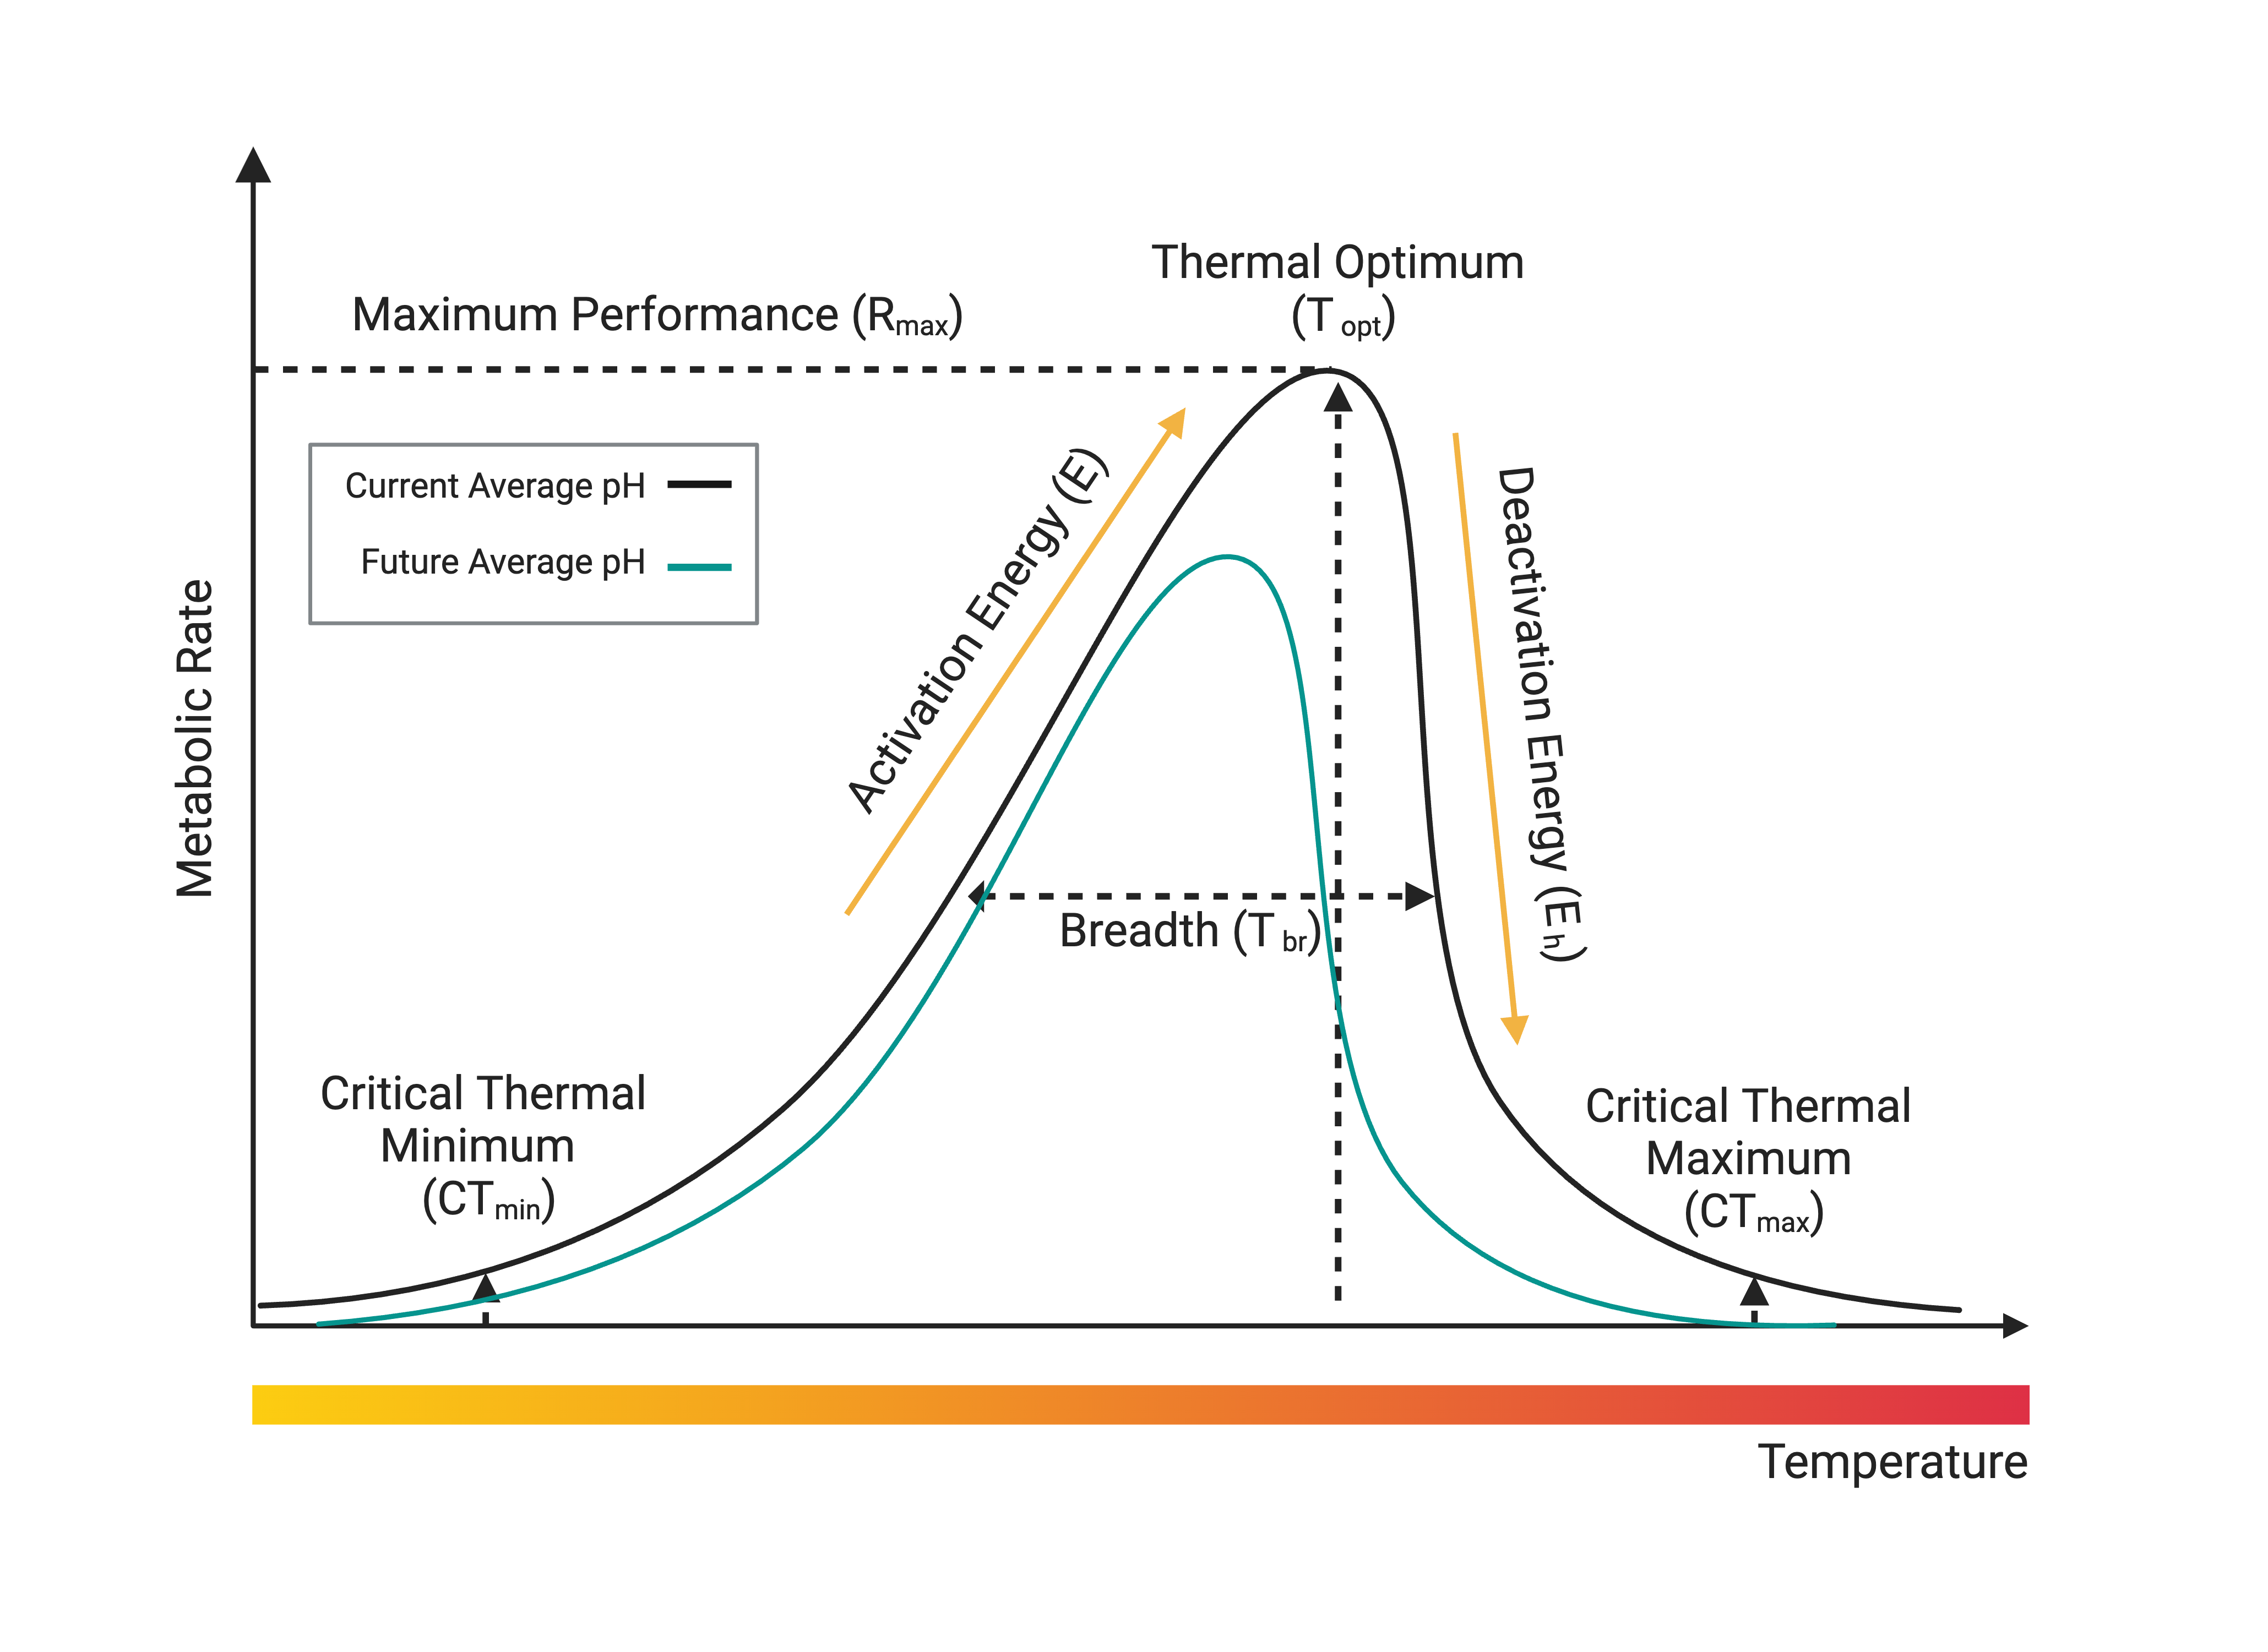
\includegraphics[width=1\textwidth]{Images/thermal_performance_curve_schematic.png}
    \caption{Figure 1. Thermal performance curve schematic illustrating the relationship between biological rates and temperature, including critical thermal maximum (CTMax), critical thermal minimum (CTMin), thermal optimum (Topt), activation energy (E), deactivation energy (Eh), and the thermal breadth of the curve (TBr). Hypothesized characteristics of a thermal performance curve exposed to ocean acidification, including reduced thermal optimum, reduced performance of maximum physiological rate, and reduced breathe of the curve.}
    \label{fig:thermal-performance-curve-schematic}
\end{figure}

~~~~~ The use of performance curves can help to quantify the
relationship between abiotic drivers and physiological rates to forecast
future effects \cite{kroeker2017embracing} and can allow for comparative
assessments across different biological rates and environmental
conditions (Figure 1.)
\cite{schulte2011thermal, silbiger2019comparative, silva2021local, padfield2021rtpc, becker2020nutrient}.
Further, thermal performance curves have been suggested to fill in the
gap of uncertainty between multiple stressors as they empirically
characterize the relationship between biological performance rates
across a wide range of temperatures
\cite{padfield2021rtpc, schulte2011thermal, silbiger2019comparative}.
Thermal performance curves are a univariate function that describes how
some measure of performance (e.g., metabolic rate) varies with
temperature. As temperature increases so do the biochemical and
physiological rates until they reach a species-specific optimal
temperature. Beyond the optimum rate, further increases in temperature
denature proteins, stunt growth, and cause reductions in performance and
survival \cite{somero2002thermal, portner2002climate}. Thermal
performance curves are typically left-skewed and hump-shaped and include
several metrics, including but not limited to a thermal optimum
(TOpt)---the temperature at the highest rate of performance---and a
critical thermal minimum (CTMin) and a thermal maximum (CTMax)--- the
upper and lower thermal limit that an organism can tolerate
\cite{schulte2011thermal, huey1979integrating, huey1989evolution}. These
tolerance thresholds and the range they encompass are governed by an
organism's ability to respond to sub-lethal and lethal conditions
through an organismal-level response and molecular-level responses such
as anaerobic metabolism and heat shock response
\cite{portner2017oxygen, somero2002thermal}. Further, exposure to
concurrent drivers of ecological change, like OA, are expected to
constrict an organism's performance curve and thermal limits, such as
decreasing the breadth of thermal performance
\cite{portner2008physiology, portner2010oxygen}. Comparing physiological
responses to gradients of abiotic drivers may allow us to quantify and
compare the tolerance limits of organisms
\cite{silbiger2019comparative}.

~~~~~ Despite the increasing emphasis on multi-driver and multi-species
studies, a mechanistic understanding of the nonlinear responses of
multiple confounding stressors of future scenarios remains a knowledge
gap. (Kroeker, Kordas, \& Harley, 2017). The elevated sense of urgency
involved with these global threats contributes to the need for a more
nuanced understanding of the impact of multiple stressor interactions on
organismal and ecosystem processes (Côté et al., 2016). The response of
organisms to climate change, survival, and fitness depends on
physiological trade-offs, which are essentially changed within the
allocation of an organism's energy for different biological functions
and demands for resources. Considering that metabolic processes respond
differently to multiple environmental drivers and that physiological
systems within and between organisms differ, it is imperative to tease
apart the metabolic rates. Organisms may respond to changing abiotic
drivers by altering their energetic allocation or energetic intake, such
as altering consumption rates or growth (O'Connor 2009). For example,
the metabolic theory of ecology predicts an increase in consumption
rates with increasing temperature (O'Connor 2009). These alterations
within an individual species' physiological performance are significant
because they can scale up to affect ecosystem function (Post et al.,
1999). Building a mechanistic understanding regarding how the combined
impacts of ocean warming and acidification affect marine organisms is
integral for reliable projections of how climate change may continue to
affect marine organisms.

~~~~~ Specifically, we ask the question: how does exposure to decreased
pH influence thermal performance curves of respiration of an intertidal
gastropod, Tegula funebralis? We anticipate that the thermal optimum
(TOpt) for respiration rates will shift towards lower temperatures,
indicating a reduced ability to sustain optimal metabolic activity in
the face of ocean acidification. Additionally, we expect a decrease in
the thermal breadth of the curve (TBr), indicating a narrower range of
temperatures at which the gastropod can effectively maintain its
respiratory rates.

\newpage

\hypertarget{methods}{%
\section{Methods}\label{methods}}

\vspace{0.5cm}

\hypertarget{a-mesocosm-design}{%
\subsection{(a) Mesocosm Design}\label{a-mesocosm-design}}

~~~~~The Silbiger Lab mesocosm system at California State University,
Northridge was used to emulate experimental conditions of a semi-diurnal
tidal fluctuation across a gradient of temperatures and blocked exposure
to either low or high pH. The facility operated as a closed-loop system,
wherein water from individual tanks was continuously recirculated back
into a central holding reservoir (sump). Unbuffered natural seawater was
collected from the Southern California Marine Institute (SCMI) in San
Pedro, CA and filtered through three mesh filters (20 \(\mu\)m, 5
\(\mu\)m, 1 \(\mu\)m) prior to being introduced into the sump of the
mesocosm system. Within the system, recirculating seawater underwent
further filtration through three 50 \(\mu\)m carbon bag filters, eight
mesh filters, a UV sterilizer (Comet Series 95 Watt Lamp), and a chiller
(Aqua Logic Delta Star, DS-4) which maintained water quality and chilled
seawater to ambient conditions. Weekly water replacements, accounting
for approximately 50\% of the total volume, were conducted to prevent
the accumulation of metabolic waste and to maintain stable carbonate
parameters within the system. The mesocosm system was equipped with 16
experimental tanks (53.9 cm (L) x 31.75 cm (W) x 34.29cm (H)) with
individual controls for temperature, light intensity, and water flow.
Each tank was outfitted with a submersible powerhead pump (Hydor Nano
Koralina 240 powerhead, 240 GPH), 200 W Heater (Hydor aquarium heater),
temperature probe (Neptune Systems, \(\pm\) 0.1\(^\circ\)C), pH probe
(Neptune Systems, Lab Grade Double Junction, measures pH from 4.0 to
12.0 \(\pm\) 0.1), three flow sensors (Apex, FS25 \(\frac{1}{4}\)''
fitting, flow rates from 3-12 GPH (12-24 LP)), and a temperature logger
(HOBO TidBit MX2203, \(\pm\) 0.2\(^\circ\)C). LED lights (Halo Basic
M-110) in each tank followed a 12:12 day/night cycle, which mimicked the
local light conditions using a sunset and sunrise table.

~~~~~Each individual tank was programmed to experience tidal
fluctuations as well as temperature/pH controlled seawater conditions
for their respective treatments. Programmable solenoid valves (Apex
Neptune) were utilized to adjust the seawater flow rates to each tank,
ensuring that either inflow rates exceeded outflow drain rates
simulating a high tide condition or outflow drain rates exceeded inflow
rates to simulate a low tide condition. This emulation aimed to
replicate the semi-diurnal tidal characteristic of the Pacific Coast.
Within a 24-hour period, two high tide and two low tide fluctuations,
each lasting six hours, were generated by either opening or closing the
solenoids. Flow rates were meticulously maintained on a daily basis
using a graduated cylinder and timepiece to ensure a programmable inflow
of 10 L/h, constant total inflow of 10 L/hour, and a constant outflow
drain rate of 15 L/hour, thereby creating the desired tidal effect.
Precise control over temperature in each tank was achieved by employing
a programmable thermostat (Neptune Apex), which automatically activated
or deactivated heaters in response to temperature deviations from the
set range. Individual tank pH levels were regulated using a pH-stat
set-up through the direct bubbling and mixing of CO2 facilitated by a pH
logger and solenoid valves (Neptune system) attached to a CO2 tank
(PhosBan Reactor 150). Additionally, in each tank, a venturi connected
to an aquarium pump facilitated the mixing of ambient air to stabilize
the pH levels in the treatment tanks. After recirculation into the sump
system, the sweater was chilled to ambient condition and scrubbed of CO2
using a phosban reactor (Phosban 150 Reactor).

~~~~~Throughout the experiment, various water quality parameters were
regularly measured to monitor environmental conditions within the tanks.
pH, dissolved oxygen (DO), and temperature were assessed daily at
consistent times to ensure accurate readings and facilitate the
calibration of in-tank temperature probes for precise measurements. pH
and dissolved oxygen levels were measured daily, within each tank using
a Termo Specific ORION ISE instrument with a resolution of 0.1 mV and an
accuracy of \(\pm\) 0.2 mV or \(\pm\) 0.05\%. Simultaneously,
temperature readings were obtained using a Thermo Fisher Trace digital
thermometer. The temperature data also aided in calibrating the
thermostat sensors within each tank, which were adjusted once a day to
maintain accurate temperature control. pH on the total scale was
calculated from mV and temperature by using a multipoint calibration to
a tris standard solution from the Dickson Lab at Scripps Institution of
Oceanography following Dickson SOP 6a \citep{dickson2007guide}. Accuracy
of the pH was tested against a Tris buffer of known pH from the Dickson
Lab at Scripps Institution of Oceanography \citep{dickson2007guide}. The
pH values for the individual aquaria were calculated using the seacarb
package in R, accounting for temperature corrections specific to each
tank \citep{gattuso2015package}. I also measured total alkalinity (TA)
from water samples collected once every few days (3-4 days) from each
experimental tank and sump. All total alkalinity (TA) water samples were
collected and stored in 125 ml Nalgene containers. Prior to use, these
containers underwent thorough cleaning in a 10\% HCl bath for 24 hours,
followed by rinsing with deionized (DI) water. Additionally, during
sample collection, the containers were rinsed three times with sample
water to ensure a representative water quality sample. Collected samples
were analyzed within 24 hours of collection using a T-5 automatic
titrator (Mettler Toledo) following the best practices for ocean CO2
measurements \citep{dickson2007guide}. To verify accuracy, a certified
reference material (Reference Material for Oceanic CO2 Measurements, A.
Dickson, Scripps Institution of Oceanography) was run prior to each
total alkalinity measurement with an error no greater than 1.0\% off
from the certified value \citep{dickson2007guide}.

\begin{table}[!ht]
    \centering
    \begin{tabular}{|c|c|c|c|c|c|}
    \hline
        \textbf{Set Temp} & \textbf{pH Treatment} & \textbf{Mean Temp C} & \textbf{Mean pH} & \textbf{Mean Salinity} & \textbf{Mean DO \%} \\ \hline
        10 & Sump & 10.94 ± 0.26 & 7.92 ± 0.04 & 32.32 ± 0.37 & 114.82 ± 1.09 \\ \hline
        12 & Ambient & 12.91 ± 0.2 & 7.95 ± 0.02 & 33.24 ± 0.11 & 113.68 ± 1.59 \\ \hline
        12 & Low & 13.17 ± 0.41 & 7.71 ± 0.03 & 32.85 ± 0.15 & 112.37 ± 1.37 \\ \hline
        14 & Ambient & 13.9 ± 0.1 & 7.97 ± 0.02 & 32.93 ± 0.07 & 106.18 ± 1.08 \\ \hline
        14 & Low & 13.7 ± 0.22 & 7.67 ± 0.01 & 32.88 ± 0.09 & 119.31 ± 2.79 \\ \hline
        16 & Ambient & 16.17 ± 0.13 & 7.93 ± 0.02 & 32.91 ± 0.07 & 102.32 ± 1.01 \\ \hline
        16 & Low & 15.92 ± 0.32 & 7.69 ± 0.02 & 32.9 ± 0.07 & 104.81 ± 6.25 \\ \hline
        18 & Ambient & 18.18 ± 0.24 & 7.91 ± 0.02 & 32.94 ± 0.07 & 99.78 ± 1.05 \\ \hline
        18 & Low & 18.38 ± 0.26 & 7.68 ± 0.02 & 32.92 ± 0.05 & 98.79 ± 1.68 \\ \hline
        20 & Ambient & 20.76 ± 0.31 & 7.87 ± 0.04 & 32.82 ± 0.07 & 103.31 ± 1.07 \\ \hline
        20 & Low & 19.62 ± 0.57 & 7.64 ± 0.02 & 32.95 ± 0.08 & 96.02 ± 5.38 \\ \hline
        22 & Ambient & 22.36 ± 0.39 & 7.84 ± 0.02 & 32.96 ± 0.07 & 98.98 ± 0.77 \\ \hline
        22 & Low & 21.64 ± 0.49 & 7.69 ± 0.01 & 32.92 ± 0.08 & 96.65 ± 1.26 \\ \hline
        24 & Ambient & 24.75 ± 0.59 & 7.82 ± 0.03 & 32.76 ± 0.13 & 102.56 ± 1.28 \\ \hline
        24 & Low & 22.88 ± 0.66 & 7.69 ± 0.02 & 32.68 ± 0.09 & 100.09 ± 1.32 \\ \hline
        26 & Ambient & 24.45 ± 1 & 7.89 ± 0.02 & 32.85 ± 0.18 & 98.99 ± 2.1 \\ \hline
        26 & Low & 25.52 ± 0.77 & 7.66 ± 0.02 & 32.99 ± 0.06 & 92.3 ± 1.59 \\ \hline
    \end{tabular}
    \caption{Table 1. Summary statistics (mean$\pm$sd) for tank treatments and associated water quality parameters subjected to low and ambient pH levels alongside temperature variations ranging from 12-26$^\circ$C. Error bars depict standard deviations, providing insights into the variability within each treatment group. The depicted parameters include temperature treatment, pH treatment, mean temperature (°C), mean pH, mean salinity, mean dissolved oxygen percentage}
    \label{meso-stat-summary}
\end{table}

\begin{table}[!ht]
    \centering
    \begin{tabular}{|c|c|c|c|c|c|c|}
    \hline
        \textbf{Set Temp} & \textbf{pH Treatment} & \textbf{Mean TA} & \textbf{Mean pCO2} & \textbf{Mean HCO3} & \textbf{Mean CO3} & \textbf{Mean DIC} \\ \hline
        10 & Sump & 2328.01 ± 25.92 & 4978230.96 ± 275963.47 & 20.26 ± 0.29 & 1.07 ± 0.06 & 21.61 ± 0.29 \\ \hline
        12 & Ambient & 2358.28 ± 19.58 & 4920188.24 ± 223654.68 & 19.13 ± 0.21 & 1.12 ± 0.04 & 20.45 ± 0.2 \\ \hline
        12 & Low & 2359.61 ± 18.06 & 4628623.06 ± 341408.31 & 10.04 ± 0.07 & 0.35 ± 0.03 & 10.58 ± 0.08 \\ \hline
        14 & Ambient & 2357.76 ± 17.16 & 2711089.29 ± 142579.38 & 10.69 ± 0.1 & 0.68 ± 0.03 & 11.49 ± 0.09 \\ \hline
        14 & Low & 2376.31 ± 22.23 & 649410.85 ± 24204.31 & 1.28 ± 0.01 & 0.04 ± 0 & 1.34 ± 0.01 \\ \hline
        16 & Ambient & 2355.87 ± 19.49 & 3363571.87 ± 164547.58 & 11.88 ± 0.11 & 0.75 ± 0.03 & 12.76 ± 0.11 \\ \hline
        16 & Low & 2350.55 ± 21.16 & 1242533.16 ± 55051.05 & 2.5 ± 0.03 & 0.09 ± 0 & 2.64 ± 0.03 \\ \hline
        18 & Ambient & 2360.54 ± 18.2 & 3843319.75 ± 202604.37 & 13.02 ± 0.12 & 0.86 ± 0.04 & 14.02 ± 0.11 \\ \hline
        18 & Low & 2409.62 ± 18.07 & 1947471.11 ± 91567.08 & 3.83 ± 0.03 & 0.15 ± 0.01 & 4.04 ± 0.03 \\ \hline
        20 & Ambient & 2348.58 ± 21.84 & 4412288.41 ± 316379.33 & 14.07 ± 0.21 & 0.96 ± 0.06 & 15.21 ± 0.2 \\ \hline
        20 & Low & 2358.68 ± 17.84 & 2840268.86 ± 137486.09 & 5.01 ± 0.04 & 0.18 ± 0.01 & 5.29 ± 0.04 \\ \hline
        22 & Ambient & 2369.09 ± 19.13 & 5298578.58 ± 240316.39 & 15.42 ± 0.13 & 1.02 ± 0.04 & 16.62 ± 0.13 \\ \hline
        22 & Low & 2358.77 ± 16.72 & 3099996.23 ± 119715.11 & 6.17 ± 0.04 & 0.28 ± 0.01 & 6.54 ± 0.05 \\ \hline
        24 & Ambient & 2356.82 ± 21.89 & 6031162.38 ± 439328.11 & 16.43 ± 0.23 & 1.14 ± 0.07 & 17.76 ± 0.21 \\ \hline
        24 & Low & 2367.69 ± 17.4 & 3745464.62 ± 190122.17 & 7.39 ± 0.05 & 0.35 ± 0.02 & 7.85 ± 0.06 \\ \hline
        26 & Ambient & 2362.64 ± 19.05 & 5523863.5 ± 327978.24 & 17.35 ± 0.23 & 1.36 ± 0.06 & 18.88 ± 0.2 \\ \hline
        26 & Low & 2350.6 ± 20.16 & 4640263.18 ± 268033.32 & 8.52 ± 0.09 & 0.42 ± 0.02 & 9.08 ± 0.09 \\ \hline
    \end{tabular}
    \caption{Table 2. Summary statistics (mean$\pm$sd) for tank treatments and associated seawater carbonate chemistry parameters subjected to low and ambient pH levels alongside temperature variations ranging from 12-26$^\circ$C. Error bars depict standard deviations, providing insights into the variability within each treatment group. The depicted parameters include mean total alkalinity (TA), mean partial pressure of CO2 (pCO2), mean bicarbonate concentration (HCO3), mean carbonate concentration (CO3), and mean dissolved inorganic carbon (DIC) computed using the seacarb package in R \citep{gattuso2015package}.}
    \label{carbonate-stat-summary}
\end{table}

\hypertarget{b-species-collection-and-maintenance}{%
\subsection{(b) Species Collection and
Maintenance}\label{b-species-collection-and-maintenance}}

\begin{figure}[htbp]
    \centering
    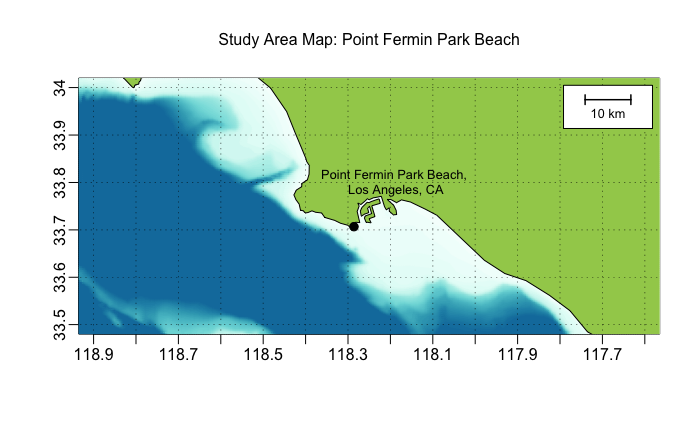
\includegraphics[width=1\textwidth]{Images/map.png}
    \caption{Figure 2. Map for study site collection located at Point Fermin State Beach (coordinates: latitude 33.7056° N, longitude 118.2935° W). Created using the Oce package \citep{kelley2018oce}.}
    \label{fig:study-site-map}
\end{figure}

~~~~~ For this experiment, black turban snails
(\emph{Tegula funebralis}) (N=80 individuals) were collected haphazardly
from tidepools in Point Fermin, San Pedro, CA (Figure 2.) on August 16,
2022 (SCP ID: S-220520002-22054-001). All collections were made and
transported during low tide to minimize any physiological variation that
might be related to endogenous tidal rhythms. Individuals of
\emph{T. funebralis} were measured for shell width (dorsal to ventral)
between 18-22 mm using Vernier calipers, since shell height is a
reliable predictor for body mass. Organisms were then transported back
to California State University, Northridge in a wet insulated container
where they were measured for blotted wet mass (g), volume displacement
(mL), shell height (mm), and shell width (mm) and tagged using a
previously weighed FloyTag placed at the apex of the dorsal side of the
shell with coraffix glue. The snails were then randomized and assigned
to an experimental treatment as detailed below. Each snail was randomly
assigned to one of 16 experimental aquaria across a range of 8
temperatures from 12-26\(^\circ\)C and two pH treatments, and placed
into their respective experimental tanks (n=4 per treatment). To adjust
the snails to their treatment temperatures, all snails started in
ambient temperature conditions (16\(^\circ\)C), and temperatures were
then increased or decreased at a rate of up to 2\(^\circ\) C per day
until reaching the set treatment temperature. The changes in pH for the
acidification treatments were simultaneously reduced with temperature
changes at a rate of up to \textasciitilde0.5 units per day during this
period as this is the fluctuation of pH that organisms in the intertidal
experience in a single day \citep{jellison2016ocean}. Organisms were
adjusted to experimental conditions for a week before the experiment
began. Throughout the experiment, snails were fed giant kelp wrack
\emph{Macrosystis pyrifera}, a highly preferred food, was collected from
Point Fermin, CA to feed organisms and placed on 3 inch PVC disks every
three days throughout the experiment. \emph{M. pyrifera} was rinsed with
fresh water to remove epiphytes prior to feeding.

\hypertarget{c-temperature-and-ph-treatment}{%
\subsection{(c) Temperature and pH
Treatment}\label{c-temperature-and-ph-treatment}}

\begin{figure}[htbp]
  \centering
  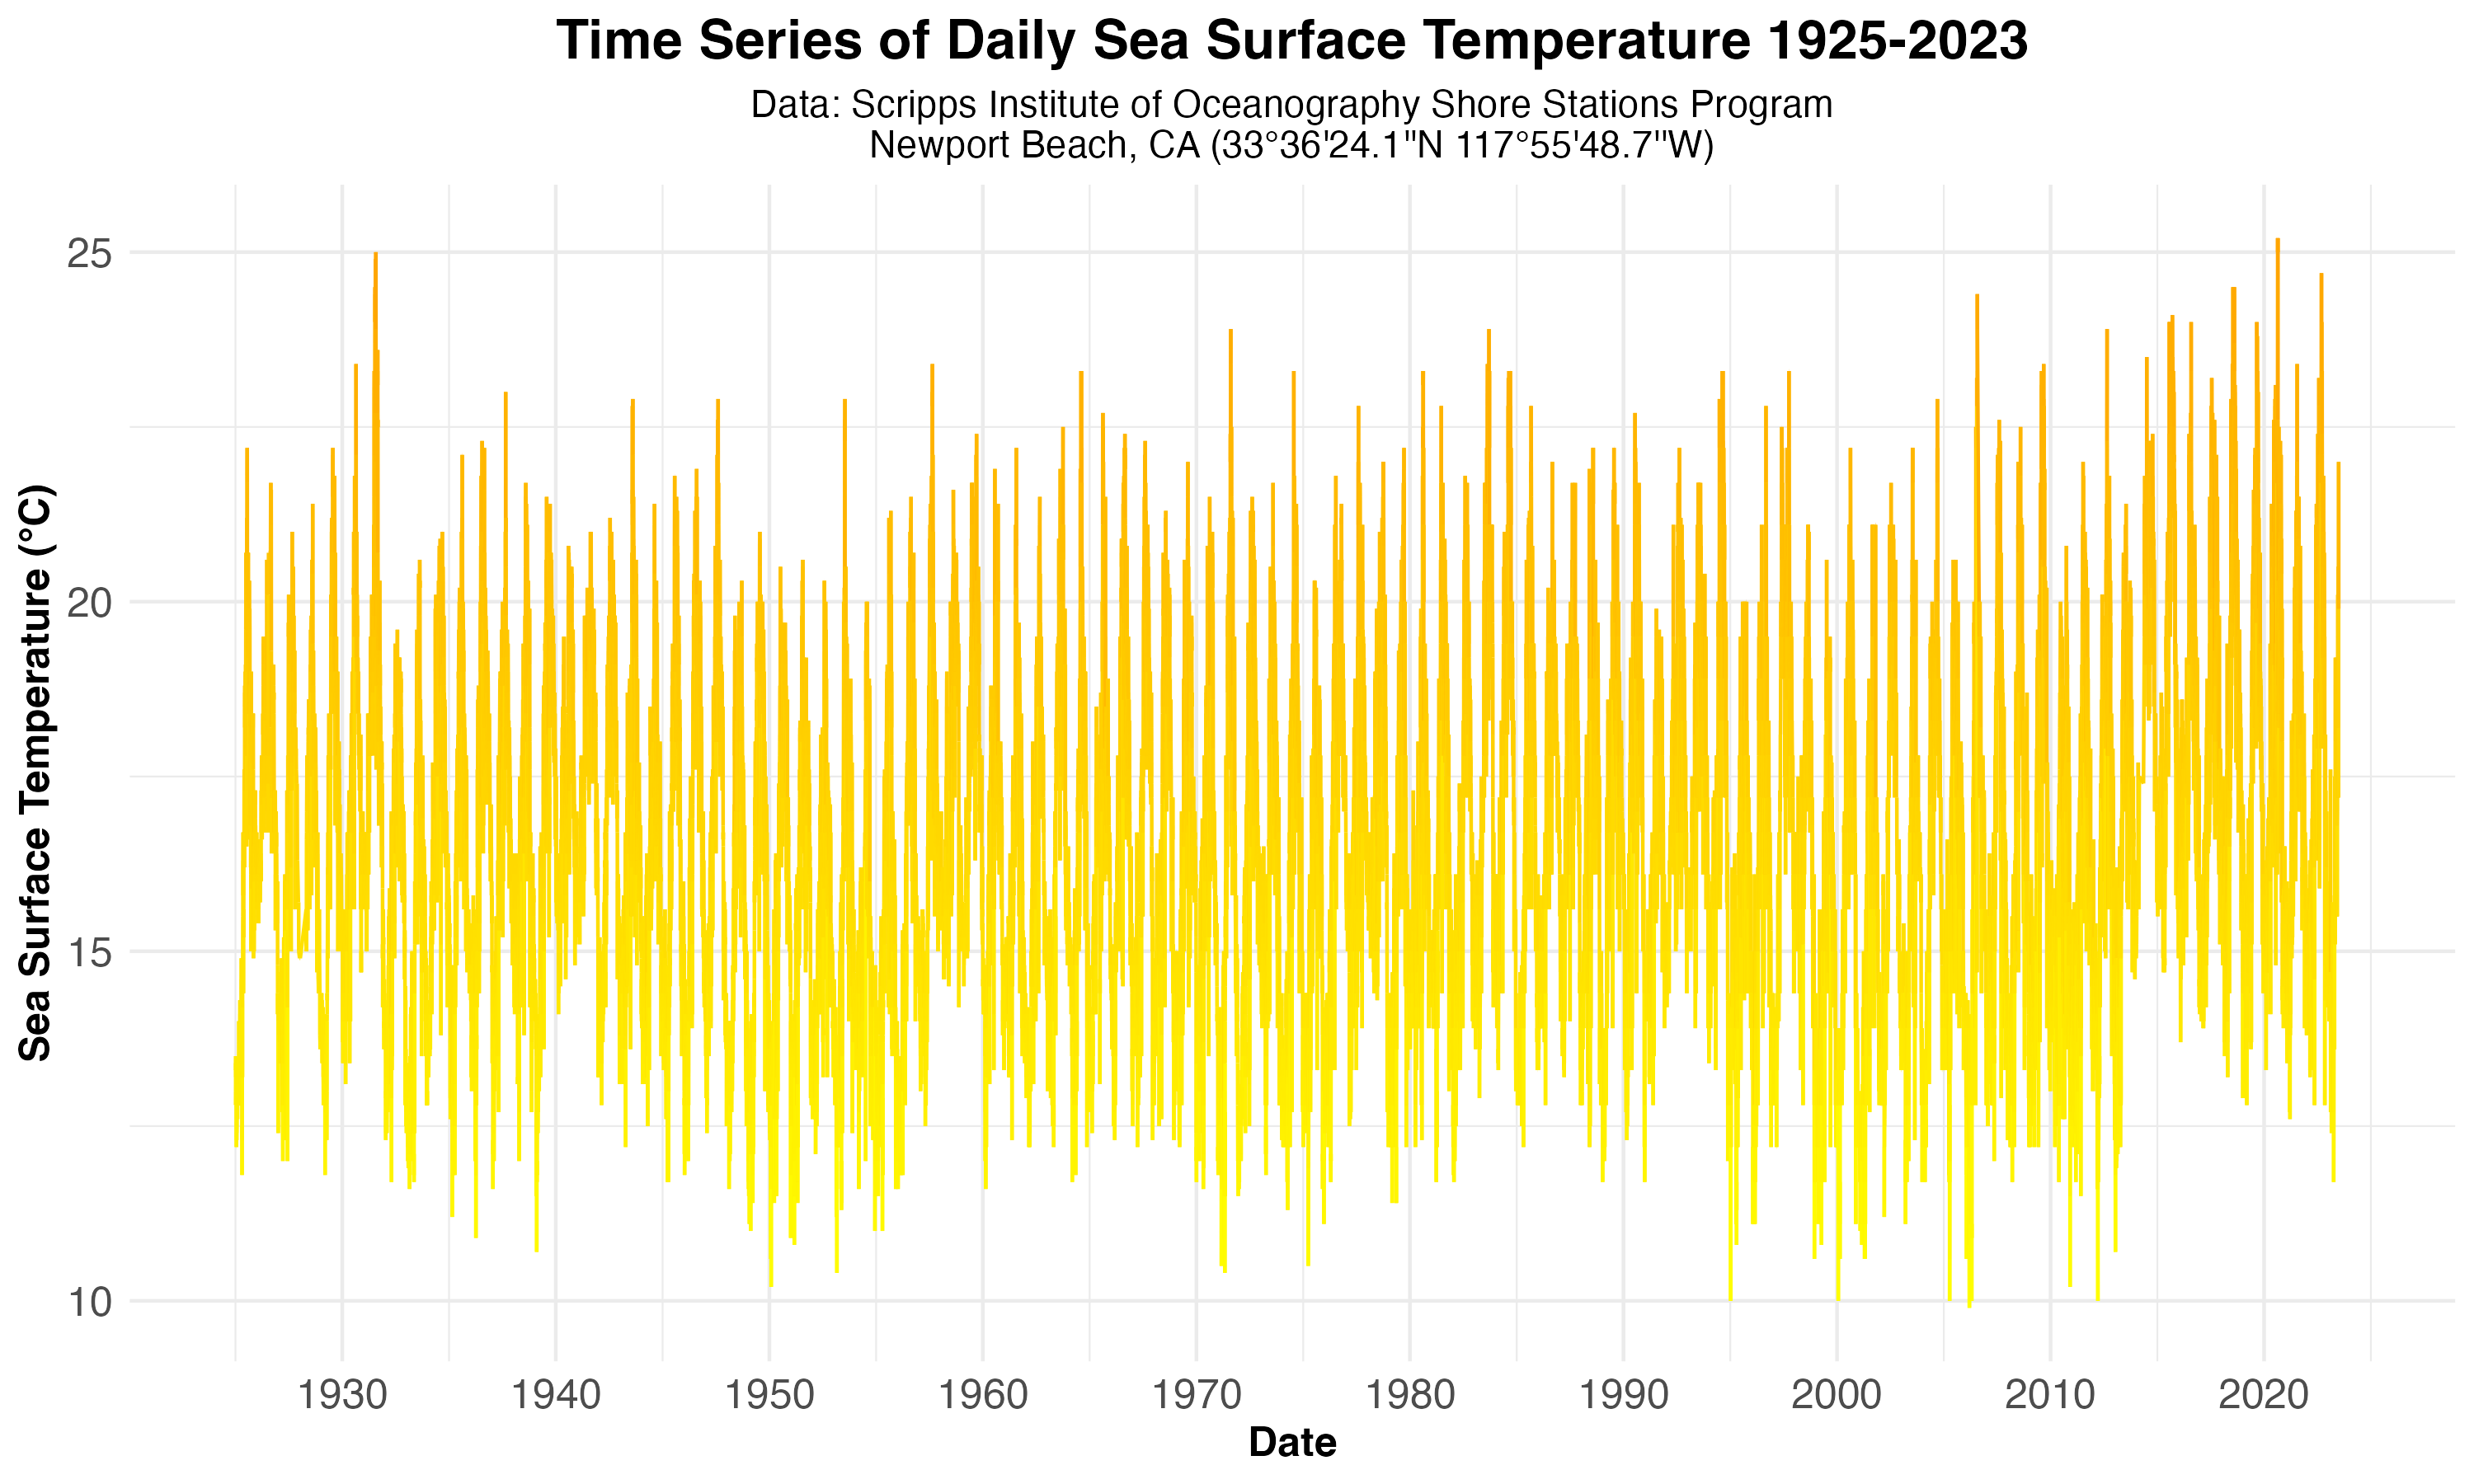
\includegraphics[width=0.8\textwidth]{Images/SST_timeseries_plot.png}
  \caption{Time series depicting the surface water sea surface temperature (SST) recorded from 1925 to 2023 at Newport Beach Pier in Newport, CA. The data were continuously collected, providing a visual representation of the daily surface temperature fluctuations near the study site. Data sourced from the UCSD Shore Stations Program \citep{carter2022shore}.}
  \label{fig:sst-timeseries}
\end{figure}

\begin{figure}[htbp]
  \centering
  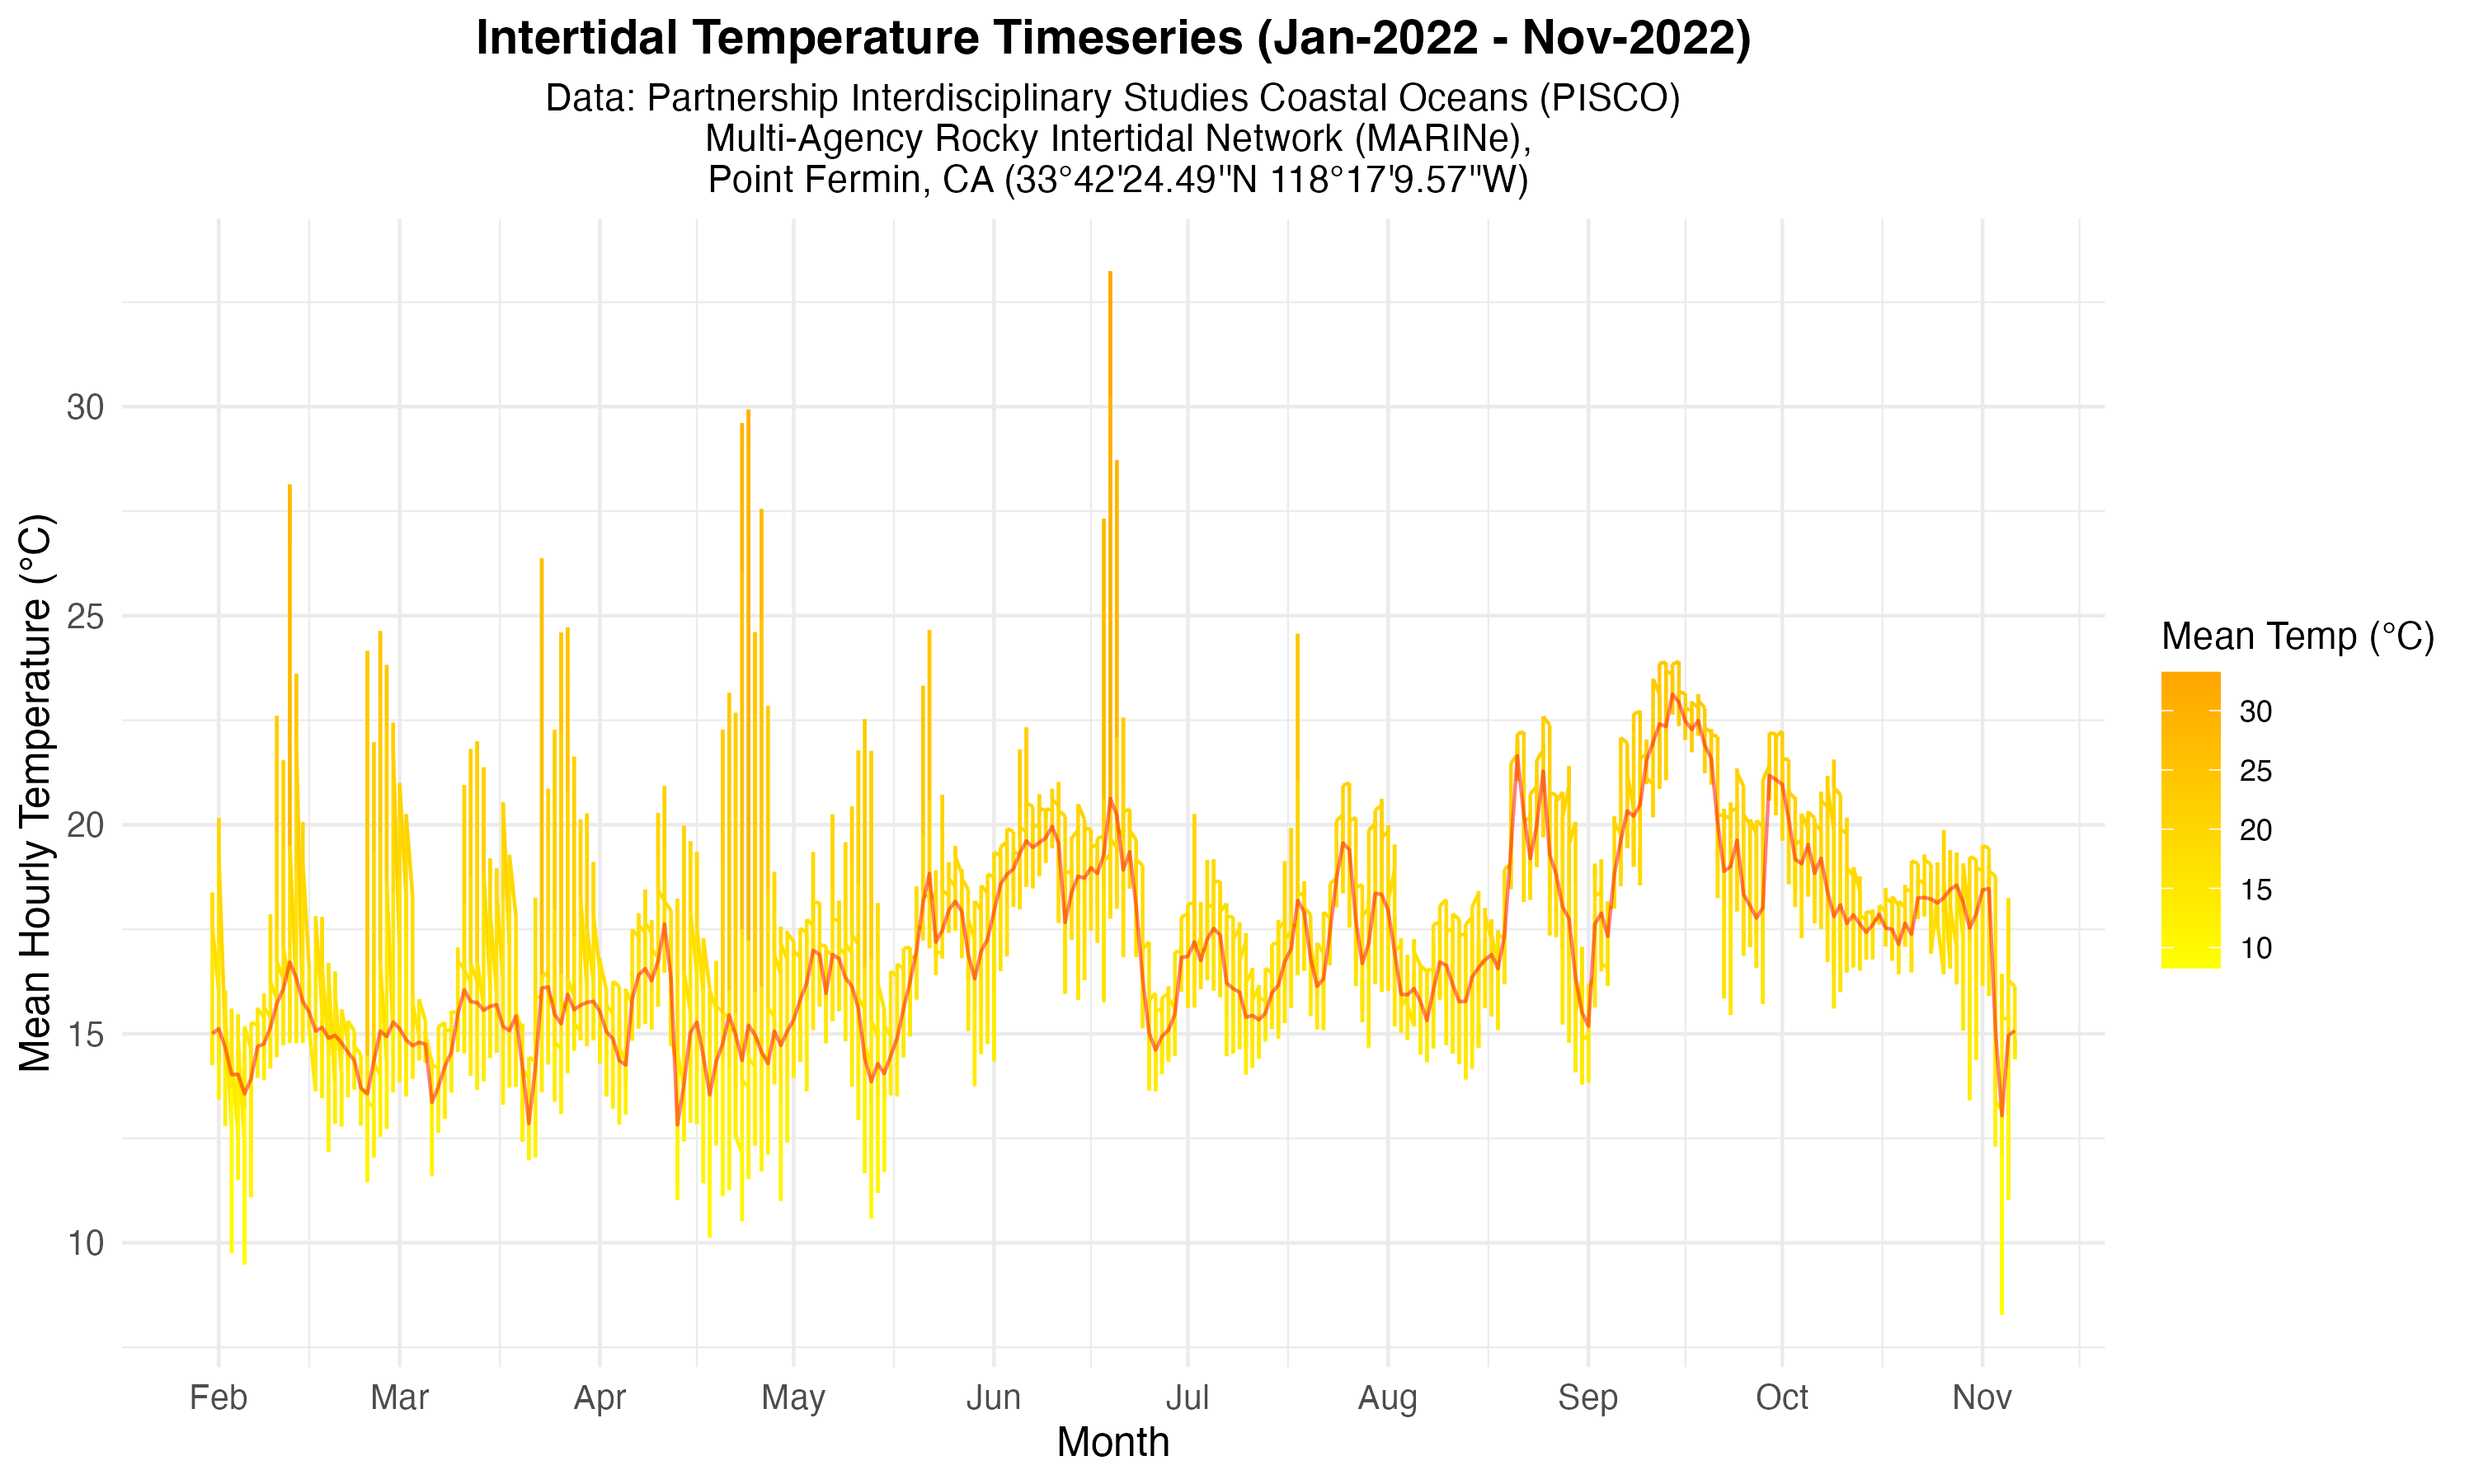
\includegraphics[width=0.8\textwidth]{Images/intertidal_timeseries_plot.png}
  \caption{Intertidal Temperature for Point Fermin, California (Data Collected Using: Onset Tidbit V2 Temp Data Logger). This figure illustrates temperature data collected from the intertidal mid zone using Onset Tidbit V2 Temp Data Logger, covering the period from January 2022 to November 2022. Data sourced from the Multi-Agency Rocky Intertidal Network (MARINe) and Partnership Interdisciplinary Studies Coastal Oceans for of (PISCO). \citep{marine_pisco_burnaford_2023}}
  \label{fig:intertidal-timeseries}
\end{figure}

\begin{figure}[htbp]
  \centering
  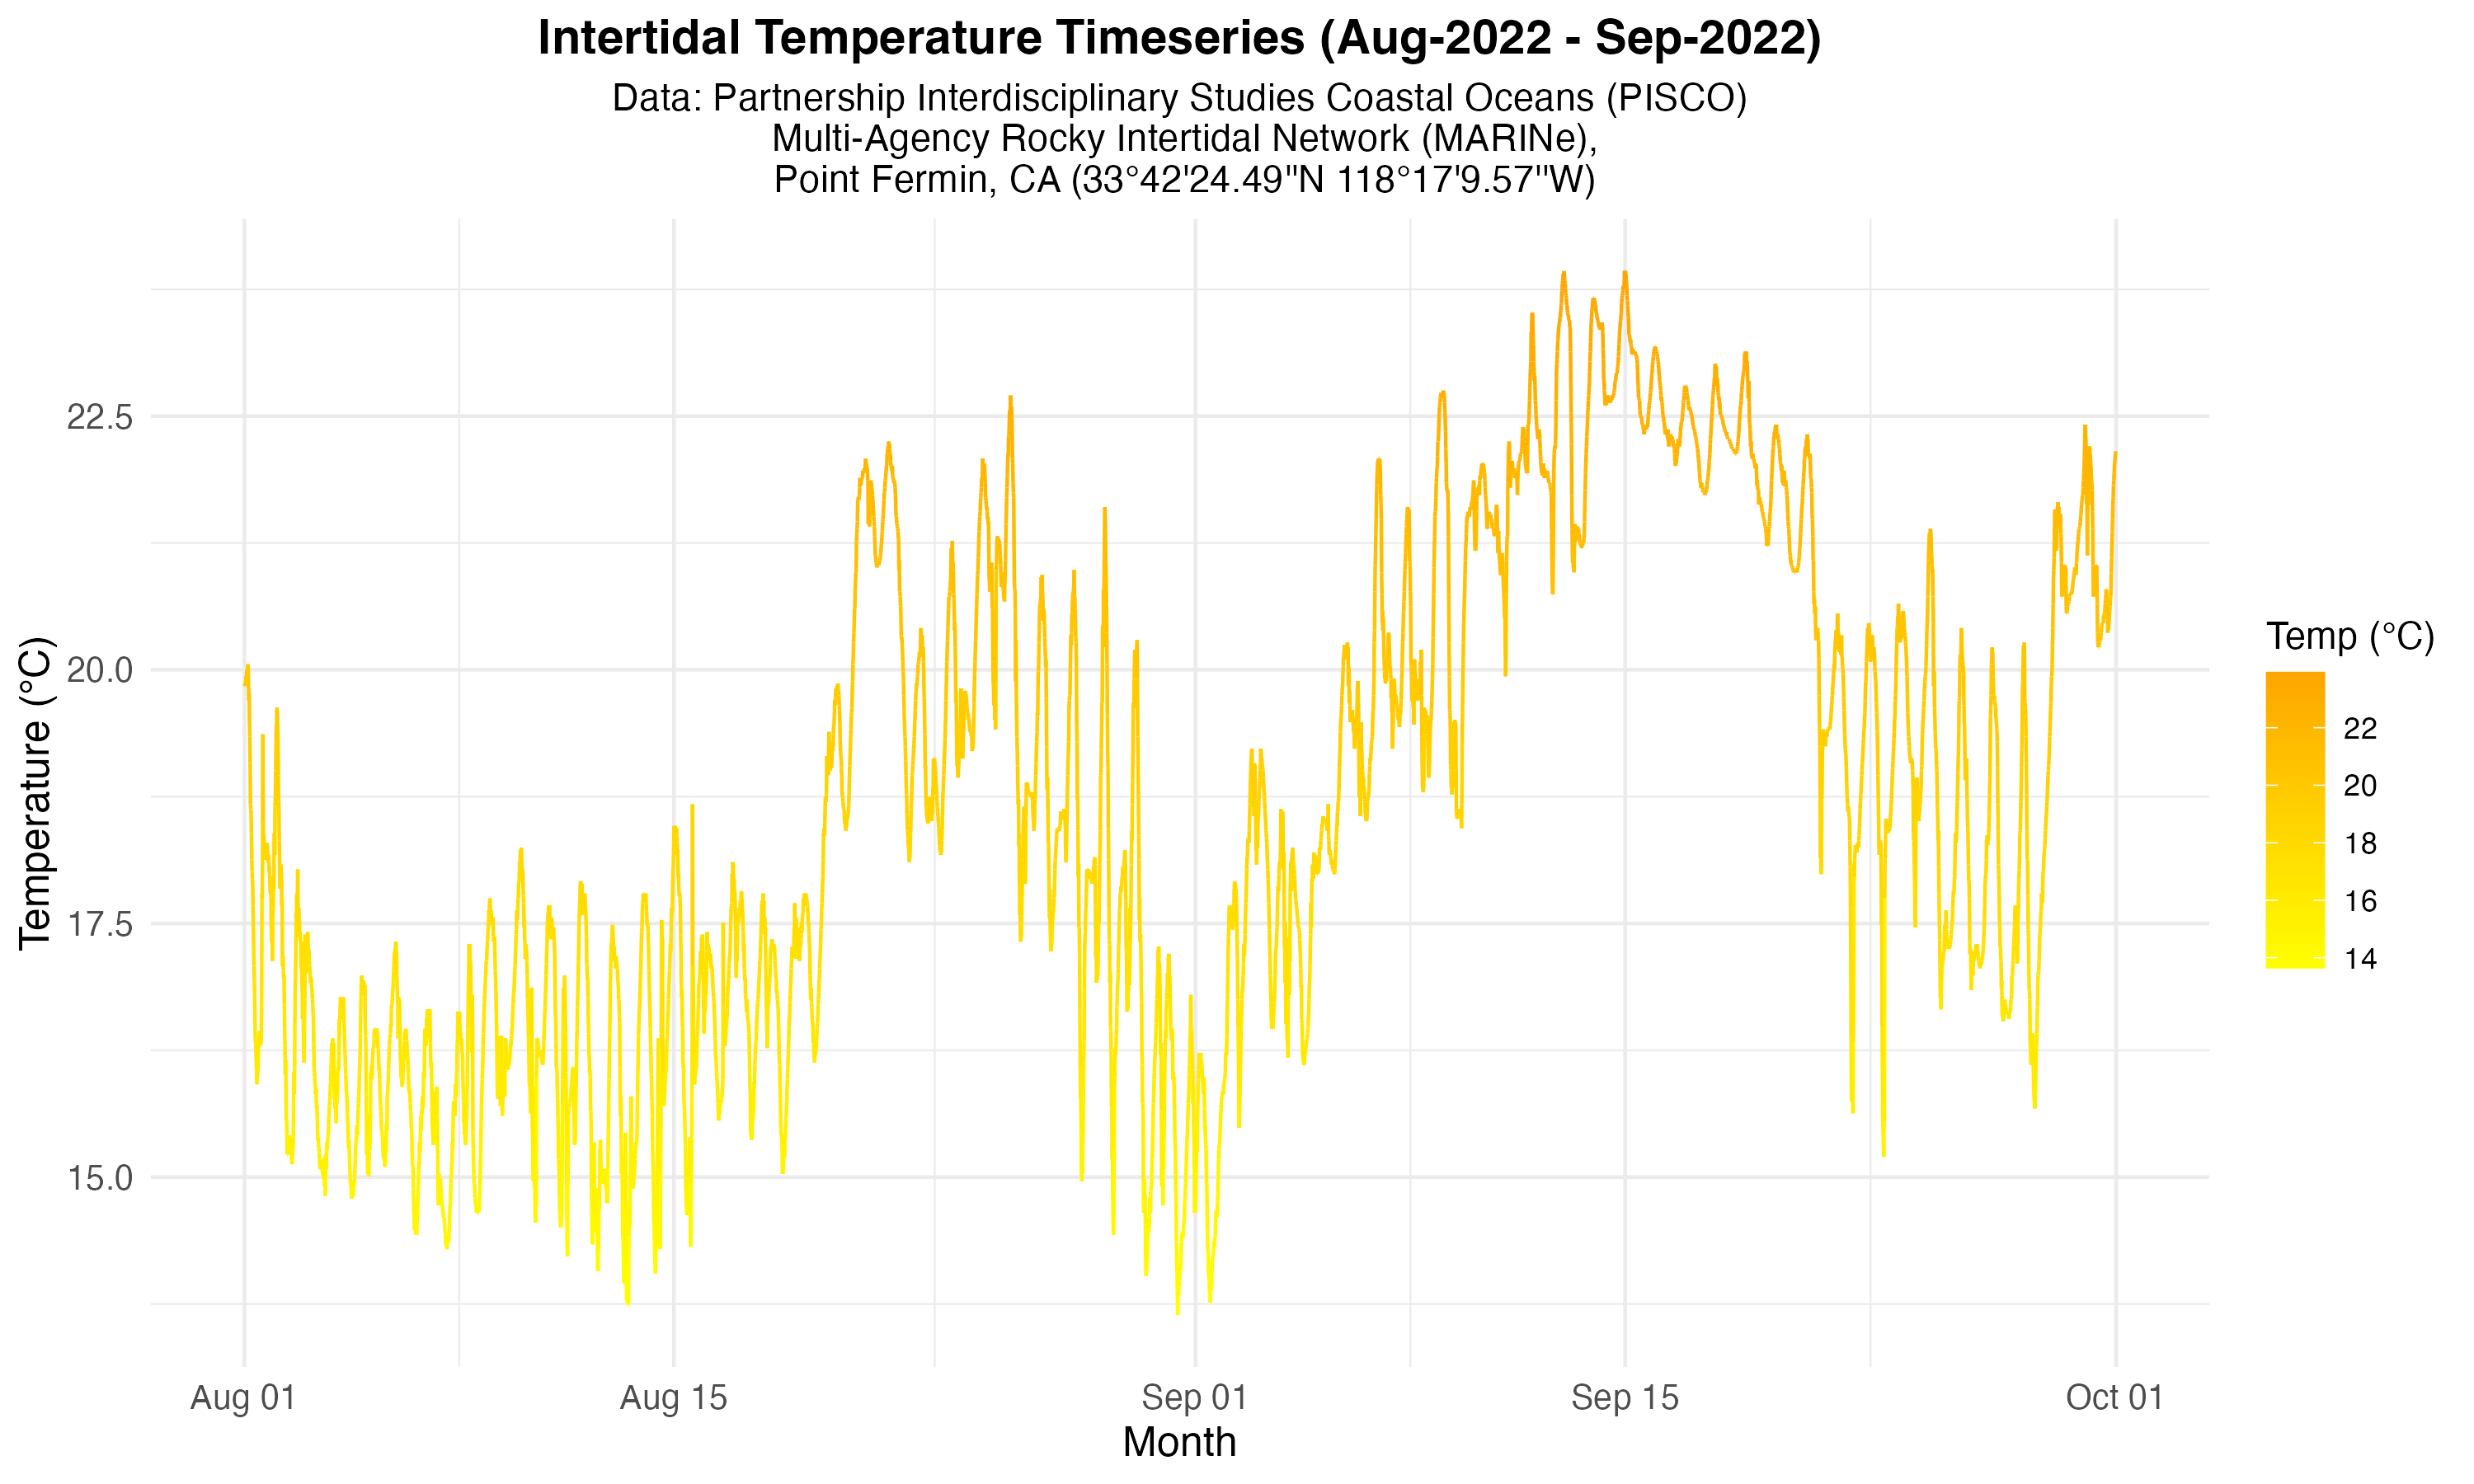
\includegraphics[width=0.8\textwidth]{Images/experiment_temp_timeseries_plot.png}
  \caption{Intertidal Temperature for Point Fermin, California (Data Collected Using: Onset Tidbit V2 Temp Data Logger) represented for August and September during the months of the experiment to visualize changes in SST. This figure zooms into the intertidal temperature dynamics during August and September, highlighting short-term fluctuations and potential impacts on intertidal organisms. Data sourced from the Multi-Agency Rocky Intertidal Network (MARINe) and Partnership Interdisciplinary Studies Coastal Oceans for of (PISCO) \citep{marine_pisco_burnaford_2023}.}
  \label{fig:intertidal-timeseries-zoom}
\end{figure}

\begin{figure}[htbp]
  \centering
  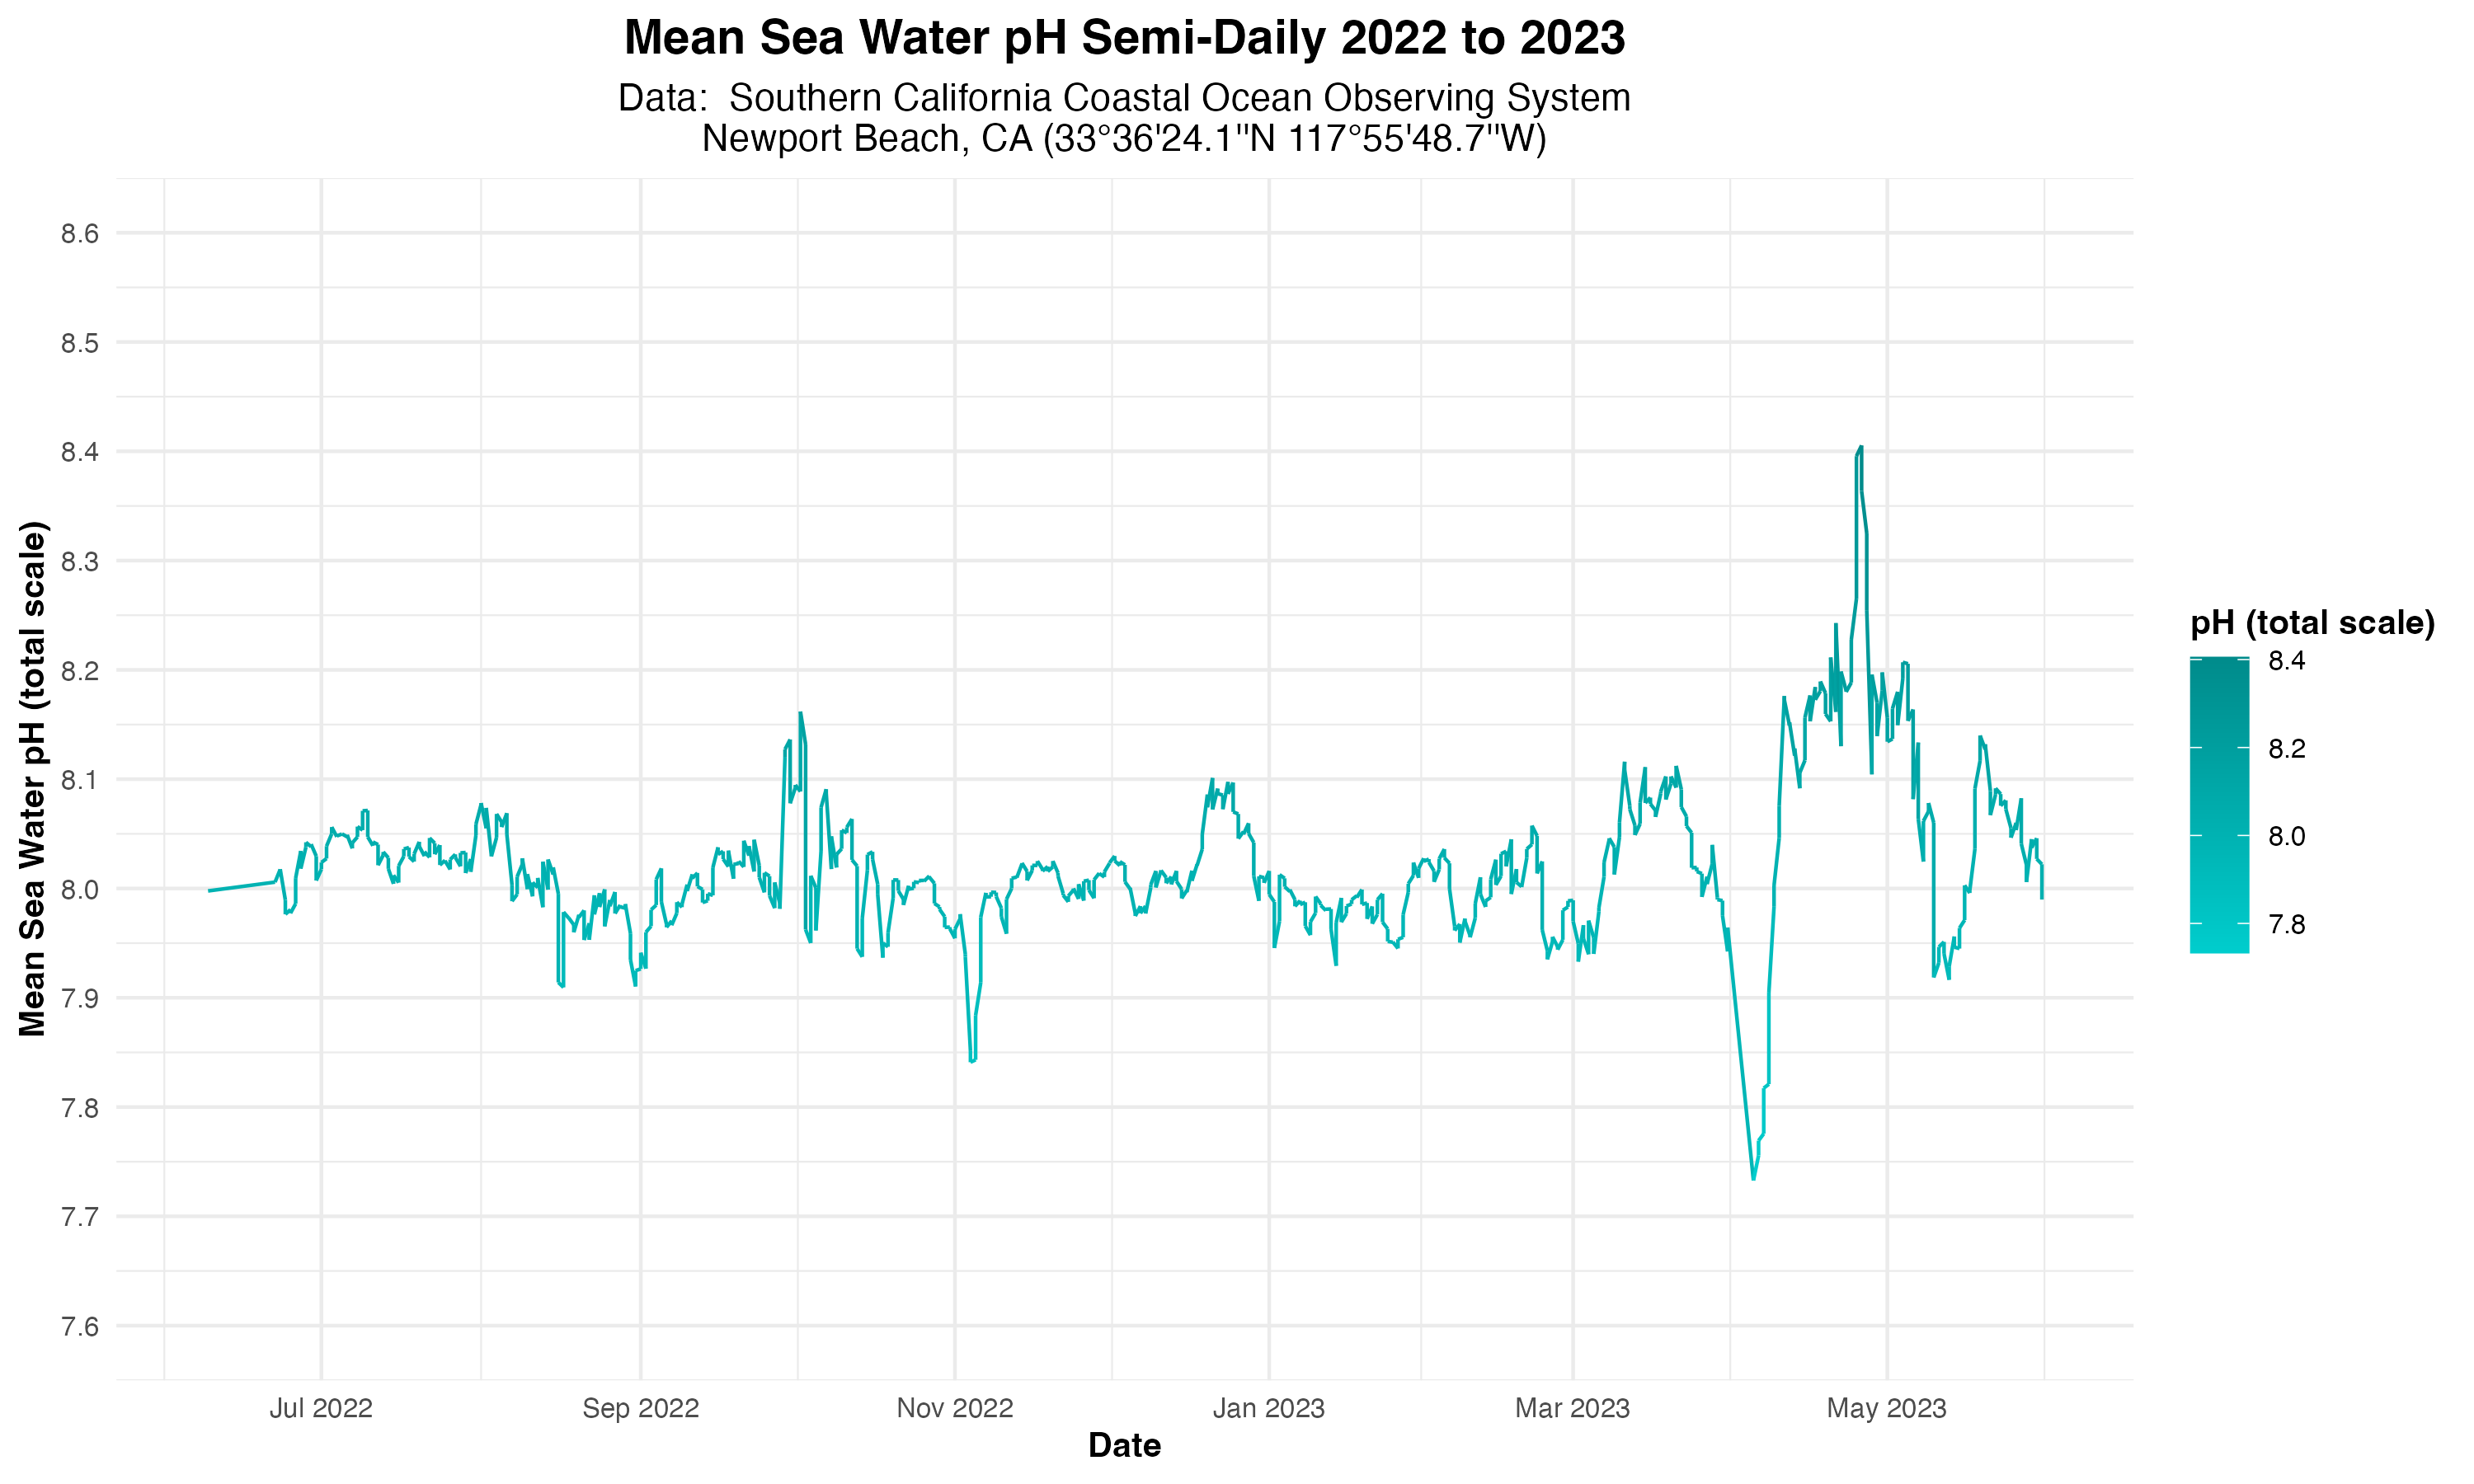
\includegraphics[width=0.8\textwidth]{Images/pH_timeseries_plot.png}
  \caption{Mean semi-daily pH (total scale) averaged every 12 hours for Newport Beach Pier in Newport, CA from 2022 to 2023. The data depict open ocean pH variability in an open shore environment without the drastic changes associated with changes in tide pool biogeochemistry. Data sourced from the Southern California Ocean Observing Systems (SCCOOS).}
  \label{fig:ph-timeseries}
\end{figure}

~~~~~ Sea snails were subjected to one of eight temperatures ranging
from 12-26\(^\circ\)C (12\(^\circ\)C, 14\(^\circ\)C, 16\(^\circ\)C,
18\(^\circ\)C, 20\(^\circ\)C, 22\(^\circ\)C, 24\(^\circ\)C,
26\(^\circ\)C; n=8) and either low or high pH conditions (7.7 or 8.0;
n=2), resulting in 16 experimental treatments. based on average facility
tank temperatures, or a realistic marine heatwave occurring on top of
ambient conditions. Nine tanks (three tanks per size class) underwent a
marine heatwave manipulation, while the remaining nine tanks were
maintained at ambient controls. Temperature conditions were chosen based
on sea surface temperature ranges and variability at a nearshore shore
station. pH was chosen due to the expected decreases of pH expected
under future conditions.

\hypertarget{d-survivorship}{%
\subsection{(d) Survivorship}\label{d-survivorship}}

~~~~~ Snail survivorship was monitored daily during the experiment.
Snails that exhibited signs of distress, such as being unable to adhere
to tank surfaces, being found at the bottom of the tank, or showing no
movement for a period of 24 hours, underwent sensory tests to assess
potential mortality. Specifically, snails were gently held w and touched
along their foot with forceps. If there was no response within thirty
seconds, they were considered deceased and subsequently removed from the
tank. Additionally, olfactory cues were also considered as indicators of
potential mortality.

\hypertarget{e-metabolic-experiment}{%
\subsection{(e) Metabolic Experiment}\label{e-metabolic-experiment}}

~~~~~ Respiration rates were measured after a 7-day adjustment period
and a 10-day exposure to the treatment conditions. Prior to conducting
respirometry, each individual snail shell was thoroughly scrubbed using
an acrylic brush to remove any epibiont communities that could
potentially obscure respiration rates. Snail respiration rates were
assessed by measuring oxygen evolution within sealed, water-tight
respirometry chambers (650 mL) for each individual. A mesh wire
separated the top and bottom sections of the chamber, with a magnetic
stir bar (200 rpms) placed in the bottom section to ensure proper mixing
of water and prevent oxygen stratification. During the respirometry
trials, temperature was carefully controlled and stabilized using an
insulated container and a programmable thermostat system (Apex
Controller, Neptune Systems \(\pm\) 0.1\(^\circ\) C). Temperature
adjustments were made using a submersible water heater (Finnex 300W
Titanium Heater) and a water chiller (Aqua Logic Delta Star, DS-4).
Oxygen measurements were taken at a frequency of 1 Hz using an oxygen
probe (Presens fiber optic oxygen dipping probe, DP-PSt8 \(\pm\)
0.1\(^\circ\) C) and continuously monitored throughout the 45-minute
respirometry trial using Presens Software. To ensure experimental
consistency, four organisms from each pH treatment (n= 8 snails) and one
blank control from each pH treatment (n = 2 blanks) were run together at
the same treatment temperature. This resulted in a total of 10
individual chambers placed in the respirometry stand and measured
simultaneously. Each chamber was fully submerged within the water bath
to maintain a controlled temperature inside. Since each respiration
chamber functioned as a sealed system, the oxygen consumption rate of
each individual organism (\((\mu mol \: O_2 \: g^{-1}h^{-1})\)) was
calculated and normalized to ash free dry weight. To obtain final wet
mass, snails were blotted with a paper towel to remove excess water,
scrubbed with a toothbrush to remove epibiont communities, and then
weighed using an electronic balance to the nearest 0.0001 g. Organic
biomass and ash free dry weight was obtained after the experiment,
during which snails were placed in a drying oven (Fisher Scientific
Isotemp Drying Oven) at 60\(^\circ\)C for 72 hours and then in a muffle
furnace (Fisher Scientific Isotemp Muffle Furnace) set to 450\(^\circ\)C
for 5 hours.

\hypertarget{f-statistical-analyses}{%
\subsection{(f) Statistical analyses}\label{f-statistical-analyses}}

~~~~~ To analyze the thermal performance curves of respiration rates and
determine the shape, we used the Sharpe Schoolfield high activation
energy model. statistical analysis was conducted in R software. The
Schoolfield model is widely used to describe the thermal performance
curves of biological rates of ectotherms. the Schoolfield model was
implemented in R to fit the data and estimate the parameters of the
model. The fitting process involved using the nmls and rTPC packages in
R to optimize the model parameters and estimate their uncertainty
\citep{padfield2021rtpc}. The data were fitted to the Sharpe Schoolfield
model (high) using AIC values between relevant performance models for
ectotherm species to evaluate the model's performance and the quality of
the fit. Furthermore, model selection techniques, such as comparing
different models based on their statistical criteria (e.g., AICc), were
employed to identify the most suitable model (e.g., gaussian,
sharpe-schoolfield low, sharpe-schoolfield full, sharpe-schoolfield
high, weibull) that accurately described the observed thermal
performance curve. Furthermore, I conducted bootstrap resampling to
estimate confidence intervals for the model predictions. \newpage

\hypertarget{results}{%
\section{Results}\label{results}}

\hypertarget{statistical-analysis}{%
\subsection{Statistical Analysis}\label{statistical-analysis}}

\subsection*{Calculation of Ash-Free Dry Weight (AFDW):}

The AFDW was determined using the following equation:

\[
AFDW = DW \times \left(1 - \frac{{\text{Ash Content}}}{{100}}\right)
\]

\begin{itemize}
    \item \( AFDW \): Ash-free dry weight.
    \item \( DW \): Dry weight of the sample.
    \item \text{Ash Content}: Percentage of ash content in the sample.
\end{itemize}

\subsection*{Conversion of Oxygen Consumption to Energy Expenditure:}

~~~~~ Cellular respiration involves the consumption of oxygen (O2)
through a process of organismal respiration to produce energy in the
form of adenosine triphosphate (ATP) \cite{babcock1992oxygen} according
to the equation:

\[
C_6H_{12}O_6 + 6O_2 \rightarrow 6CO_2 + 6H_2O + \text{energy (as ATP)}
\]

~~~~~ To calculate respiration, we first multiplied the moles of oxygen
consumed per hour by the molar mass of oxygen, which is approximately
\(32 \, \text{g/mol}\) \citep{hochachka1983protons}, to convert from
moles of oxygen to grams of oxygen. Then we used an oxy-joulometric
conversion factor derived from \cite{elliott1975energy}, which is
\(14.14 \, \text{J/mg O}_2\), to convert from grams of oxygen consumed
per hour to joules of energy expended during cellular respiration.

The calculation can be expressed as follows:

\[
\text{Energy expenditure (J)} = \text{grams of O}_2 \times \text{conversion factor}
\]

To convert moles of oxygen to grams, we used the molar mass of oxygen:

\[
\text{grams of O}_2 = \text{moles of O}_2 \times 32 \, \text{g/mol}
\]

Substituting the values, we get:

\[
\text{Energy expenditure (J)} = \text{grams of O}_2 \times 14140 \, \text{J/g O}_2
\]

where \(32 \, \text{g/mol}\) is the molar mass of oxygen and
\(14140 \, \text{J/g O}_2\) is the conversion factor derived from
\cite{elliott1975energy} and expressed as \(14.140 \, \text{J/mg O}_2\)
before conversion.

~~~~~ After converting the oxygen consumption rates to energy
expenditure in joules per hour per snail and performing statistical
analysis, we conducted a two-way ANOVA to investigate the effects of
temperature treatment and pH treatment on energy expenditure. The ANOVA
revealed a significant effect of temperature treatment (\(p < 0.001\)),
indicating that different temperature treatments had a significant
impact on energy expenditure. Although the pH treatment showed some
effect on energy expenditure, it was marginally significant (F(1, 44) =
3.9760, p = 0.05237), suggesting a potential influence of pH on energy
expenditure. The interaction between temperature and pH treatment was
not significant (F(7, 44) = 1.5286, p = 0.18280), indicating that the
combined effect of temperature and pH treatment did not significantly
impact energy expenditure beyond the individual effects of each factor.
Subsequent Tukey multiple comparisons showed significant differences
between most temperature treatment pairs. For example, the energy
expenditure at 14°C was significantly higher than at 12°C (mean
difference = 13.31 J/h, p \textless{} 0.001), and the energy expenditure
at 22°C was significantly higher than at 20°C (mean difference = 60.21
J/h, p \textless{} 0.001). Tukey multiple comparison indicated a
significant difference between low and ambient pH conditions, with a
higher energy expenditure observed under low pH (mean difference = 5.95
J/h, p \textless{} 0.001).

\begin{table}[htbp]
    \centering
    \caption{Energy Expenditure at Different Temperatures for Ambient and Low pH Treatments}
    \label{table3}
    \begin{tabular}{cccc}
    \toprule
    Temperature & Treatment & Energy Expenditure (J/h) & Percent Difference \\
    \midrule
    12 & Ambient & 20.68363 & -10.28\% \\
    & Low & 23.05466 & \\
    14 & Ambient & 33.82566 & -8.28\% \\
    & Low & 36.88008 & \\
    16 & Ambient & 33.41744 & -19.53\% \\
    & Low & 41.52857 & \\
    18 & Ambient & 68.02335 & 19.56\% \\
    & Low & 56.89424 & \\
    20 & Ambient & 69.03278 & -4.30\% \\
    & Low & 72.13377 & \\
    22 & Ambient & 58.85060 & -37.60\% \\
    & Low & 94.31767 & \\
    24 & Ambient & 85.51626 & -20.26\% \\
    & Low & 107.24288 & \\
    26 & Ambient & 53.82479 & -5.62\% \\
    & Low & 57.03218 & \\
    \bottomrule
    \end{tabular}
\end{table}

\newpage

\subsection*{Thermal Performance Curve Analysis:}

~~~~~ All statistical analyses were run in the R environment
\citep{R_core_team_2021}. The \textit{rTPC} \citep{padfield2021rtpc} and
\textit{nls.multstart} packages were used to fit a series of models to
the respiration rate data and build thermal performance curves. The
analysis utilized the \textit{rtpc} package in R, which enables a
pipeline to fit data to multiple models simultaneously. Thermal
performance curves (TPC) were analyzed to investigate the relationship
between temperature and performance measure (e.g., metabolic rate) of
\textit{T. funebralis}. The statistical processing of the thermal
performance curves involved analyzing the data collected from the
respiration chambers and examining statistical graphs of oxygen
evolution over time. Regression analysis was employed to explore the
relationship between temperature and oxygen evolution and to estimate
the parameters of the thermal performance curve (e.g., slope).
Specifically, we have utilized techniques such as nonlinear regression
to fit thermal performance models to the data and assess the goodness of
fit.

~~~~~ During the regression analysis, it was crucial to examine the
distribution of model parameters this involved assessing the normality
of the distribution of \(\beta\) values and investigating potential
outliers or unusual patterns.Additionally, we inspected the distribution
of residuals, which are the differences between observed and predicted
values, to ensure they were normally distributed and exhibited
homoscedasticity. Additionally, diagnostic plots, specifically
quantile-quantile (Q-Q) plots, were employed to assess the normality of
residuals and identify any potential outliers or systematic patterns
embedded within the data. We examined the relationship between predictor
variables (e.g., temperature) and fitted values to ensure the model
adequately captured the underlying trends in the data. Moreover, we
inspected the standard residuals, to identify observations with
unusually large or small residuals. Any outlying observations that
indicated data errors, measurement inaccuracies, or other anomalies that
necessitated further investigation were subsequently excluded from the
analysis.

\newpage

\subsection*{Model Fit and Selection:}

~~~~~ The thermal performance curve (TPC) model was fitted to the data
using nonlinear regression techniques in R, specifically the
\texttt{nls\_multistart()} function. Model fit was assessed with the
coefficient of determination (\(R^2\)), indicating a strong fit to the
observed data. The model selection process involved fitting several
models for ectotherm physiology (e.g., Gaussian, Sharpe-Schoolfield)
using Akaike Information Criterion corrected for small sample sizes
(AICc). The Sharpe-Schoolfield model was chosen as the preferred model
for this study due to its goodness of fit, and its physiological
relevance to ectotherms based on enzyme kinetics. This model is widely
used in ecological and physiological studies to understand how organisms
respond to changing environmental temperatures, particularly in the
context of climate change and thermal stress.Additionally, bootstrap
resampling methods were employed to assess parameter uncertainty and
validate the uncertainty of the data following
\cite{Olito2017estimating}.

\textbf{Sharpe-Schoolfield High Model Equation:} \begin{equation}
R(T) = \frac{R_{\text{ref}}}{1 + e^{\left(\frac{E}{k}\left(\frac{1}{T} - \frac{1}{T_{\text{ref}}}\right)\right) + e_h\left(\frac{1}{T} - \frac{1}{T_{\text{opt}}}\right)}}
\end{equation}

\textbf{Description of Variables:}

\begin{itemize}
    \item \( R(T) \): Rate of the biological process at temperature \( T \).
    \item \( R_{\text{ref}} \): Rate at the standardised temperature, \( T_{\text{ref}} \).
    \item \( E \): Activation energy (eV).
    \item \( k \): Boltzmann's constant (\( 8.617333262145 \times 10^{-5} \) eV/K).
    \item \( T \): Temperature (°C).
    \item \( T_{\text{ref}} \): Standardisation temperature (°C). Temperature at which rates are not inactivated by either high or low temperatures.
    \item \( e_h \): High temperature deactivation energy (eV).
    \item \( T_{\text{opt}} \): Temperature (°C) at which enzyme is 1/2 active and 1/2 suppressed due to high temperatures.
\end{itemize}

\textbf{Additional Information:} The Sharpe-Schoolfield high model
describes the temperature dependence of biological rates, such as
metabolic rates, enzyme activities, or reaction rates, in response to
high temperatures. It incorporates parameters such as activation energy,
high temperature deactivation energy, and optimum temperature to
characterize the thermal performance curve \cite{sharpe1981non}. The
results of the thermal performance curve analysis provide insights into
the organism's temperature-dependent performance and its thermal
ecology. The optimum temperature (Topt) indicates the temperature range
in which the organism performs optimally, while the thermal limits
(CTmin and CTmax) define the species' thermal tolerance. The thermal
sensitivity or breadth parameter (b) reflects the organism's ability to
acclimate or adapt to temperature changes and its vulnerability to
thermal stress.

\begin{figure}[htbp]
  \centering
  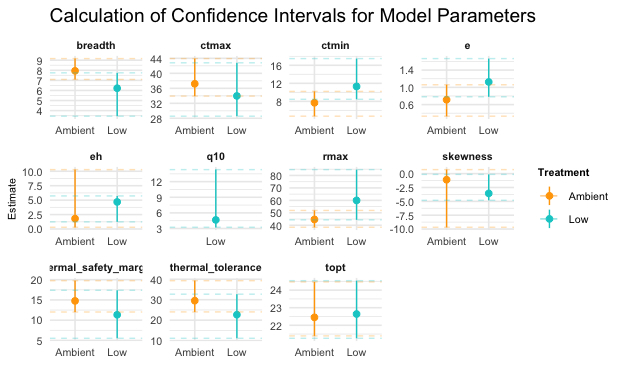
\includegraphics[width=0.8\textwidth]{Images/params.jpg}
  \caption{Extracted thermal performance parameters and metrics for \textit{Tegula funebralis}, indicating no statistical difference between the thermal performance curves (TPCs) under ocean acidification (OA) treatment overall for all TPC parameters.}
  \label{fig:tpc-params}
\end{figure}

\begin{figure}[htbp]
  \centering
  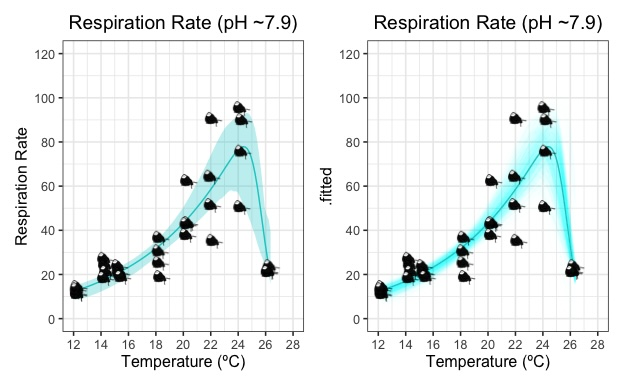
\includegraphics[width=0.8\textwidth]{Images/schoolfield-high.jpg}
  \caption{Thermal performance curve of \textit{Tegula funebralis}, depicting individuals' respiration rates (in $\mu mol$ O$_2$ per gram of ash-free dry weight) across temperatures ranging from 12°C to 26°C at a pH of 7.9 $\pm$ 0.1. One plot includes bootstraps while the other presents calculated confidence intervals. The plot was generated using the \texttt{rtpc} package in R \citep{padfield2021rtpc}.}
This caption provides a clear description of the figure, including the species studied, the 
  \label{fig:tpc-schoolfield-high}
\end{figure}

\begin{figure}[htbp]
  \centering
  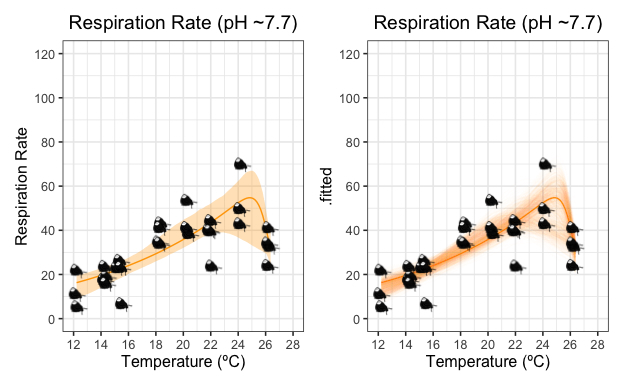
\includegraphics[width=0.8\textwidth]{Images/schoolfield-low.jpg}
  \caption{Thermal performance curve of \textit{Tegula funebralis}, depicting individuals' respiration rates (in $\mu mol$ O$_2$ per gram of ash-free dry weight) across temperatures ranging from 12°C to 26°C at a pH of 7.7 $\pm$ 0.8. One plot includes bootstraps while the other presents calculated confidence intervals. The plot was generated using the \texttt{rtpc} package in R \citep{padfield2021rtpc}.}
  \label{fig:tpc-schoolfield-low}
\end{figure}

\newpage

\hypertarget{discussion}{%
\section{Discussion}\label{discussion}}

Better understanding the impacts of global climate change on marine
ecosystems requires us to think outside the confines of direct impacts
(Kroeker et al., 2012) since individual alterations in organismal
physiology have much larger implications for communities (Kroeker et
al., 2012; Gaylord et al., 2015).These results presented in this thesis
highlight the importance of considering the physiological and
geochemical interactions between temperature and carbonate chemistry
when interpreting species' vulnerability to OA, as multiple drivers of
ecological change may interact in myriad ways. This study also
illustrates the use of thermal performance curves as a mechanistic way
to tease apart multiple drivers of ecological change to make more
accurate predictions of species' vulnerability to future climate
change.Understanding changes in metabolic rates to different magnitudes
and combinations of abiotic drivers may elucidate complex changes in
physiological mechanisms that are unable to be uncovered using a few
treatments (Becker and Silbiger, 2020; Edmunds et al., 2011).

urther, assessing the interactive effects warming and pH using a
performance curve approach may help us better understand how performance
curves change shape with the inclusion of other abiotic factors, which
have been explored through other mechanistic approaches such as the
Oxygen and Capacity-Limited Thermal Tolerance concept (Pörtner, et
al.~2017). Therefore, performance curves should be utilized through a
comparative lens to better understand the role that pH has on thermal
performance to create novel approaches to quantify and categorize
performance under a range of pH conditions.It is expected that ocean
acidification will impose additional energetic costs through
physiological stress and therefore narrow the breadth and optimum of the
curve (Pörtner 2008; Gaylord et al., 2015). The ability for organisms to
respond to anthropogenic-induced acidification depends on species level
acid- base regulation and will result in increased energy demand and
respiration rates (Pörtner, 2008). Measuring organism responses to a
range of pH in the presence or absence of thermal stress may also
provide information regarding how temperature may impact performance
under differing pH environments.

One possible explanation for this phenomenon is that the increased
metabolic rate exhibited by \textit{T. funebralis} serves as a
compensatory response to the adverse conditions induced by ocean
acidification. In the case of \textit{T. funebralis}, it is plausible
that the species is augmenting its metabolic rate as a means of
upholding vital functions and maintaining homeostasis amidst acidic
conditions. Another mechanism could be the upregulation of metabolic
pathways that generate ATP, the energy currency of cells, to meet the
increased energy demands at higher temperatures. This is consistent with
the findings of other studies that have shown elevated metabolic rates
in gastropods or decreases in body size associated with increased
temperture Ccitation). Turban snails found at lower latitudes of the
coastline grow smaller at a faster rate as well as live longer than
those found at higher latitudes (Frank, 1975); falling in line with the
metabolic theory of ecology and the expected decrease in body size under
higher temperatures (Brown et al., 2004). Research by Elahi (2020)
illustrates decreasing gastropod shell size over the past few decades
and expectations for changes in the future. It is therefore imperative
to understand the direct and indirect implications of shrinking shell
sizes on organisms.

The present study found that the respiration rate of
\textit{T. funebralis} is highly dependent on temperature, with the
highest respiration rate occurring between 20-22°C, consistent with
other thermal performance studies of the species (somnero). The present
study also found that the effects of OA on respiration rate are highly
dependent on temperature. Although high CO\(_2\) increased respiration
rate at 20°C, this effect gradually lessened with successive warming to
20°C, illustrating how moderate warming might be able to mediate the
effects of OA through temperature's effects on both physiology and
seawater geochemistry. Furthermore, other studies on the energy budget
and transfer of \textit{Tegula funebralis} indicate that rates of
aquatic and aerial respiration differ, with low intertidal individuals
respiring at a rate of 75 µl O\(_2\)/hr in water and 43 µl/hr in air
cite(paine1969). The large- scale spatial gradient and relatively
heterogeneous environment of the Pacific coast, as well as the wide
biogeographic distribution of the Tegula genus species specific
evolution to particular zonations make them the Darwins finches of
thermal ecology. It has been found that \textit{T. funebralis} has a
wider thermal tolerance range compared to its congeners,
\textit{T. brunnea} and \textit{T. montereyi}, which inhabit lower
intertidal and subtidal zones \cite{tomanek1999evolutionary}. However,
this is precisely what might make \textit{T. funebralis} more vulnerable
to future changes of a few degrees as it already withstands drastic
temperature fluctuations within the intertidal.

This study lso discovered that there will be changes in the energy
budget of \textit{Tegula} as a result of ocean acidification and
warming, which could have consequences on other specie in the
intertidal. Slight changes within the energy budget of this ubiquitous
species could have downstream consequences in terms of energy transfer,
as the rate of annual consumption by \textit{Tegula} is estimated to be
1,071 kcal m\(^{-2}\) yr\(^{-1}\) while the net primary production is
estimated to be about 1,167 kcal m\(^{-2}\) yr\(^{-1}\), with about 60\%
of energy transferred, illustrating the important role \textit{Tegula}
play in both balancing intertidal ecosystems but also in transferring
energy throughout the ecosystem cite(paine19710). The
macroalgal-herbivore interaction,is of prime importance as it is the
primary pathway for energy to move through trophic levels and is
predicted to change under projected ocean warming and acidification
(O'Connor et al., 2009). Alterations within metabolic rates of
performance such as respiration, calcification, and growth attributed to
climate change will ultimately affect net ecosystem production, net
ecosystem calcification, and food web dynamics. \newpage

\hypertarget{conclusion}{%
\section{Conclusion}\label{conclusion}}

\newpage

\bibliography{bibliography}

\newpage

\hypertarget{appendixces}{%
\section{Appendix(ces)}\label{appendixces}}

A last section may contain supporting data for the text in the form of
one or more appendices. Appendices should be placed after the
bibliography. The appendices must fall within the margin requirements
and may be single-spaced if necessary. The ETD website gives students
the option to upload ``Supporting Files'' in addition to the
thesis/dissertation. Supplemental files can include large appendix type
material, videos, images, audio files, PowerPoint presentations, and any
other file type, which will not be embedded into the main thesis
document.

\hypertarget{appendix-a-additional-tables}{%
\subsection{Appendix A: additional
tables}\label{appendix-a-additional-tables}}

Insert content for additional tables here.

\newpage

\hypertarget{appendix-b-additional-figures}{%
\subsection{Appendix B: additional
figures}\label{appendix-b-additional-figures}}

Insert content for additional figures here.

\newpage

\hypertarget{appendix-c-code}{%
\subsection{Appendix C: code}\label{appendix-c-code}}

Insert code (if any) used during your dissertation work here.

\end{document}
